% =====================================================================
%  final_report.tex   —   FORGE INFO 698 FINAL REPORT
%
%  FORMAT: this document IS the approved proposal, extended. Sections 1-4
%  are the proposal carried forward unchanged; Sections 5-9 are new
%  (verdict, research component, results, discussion, conclusion);
%  Sections 10-12 are the proposal's ethics / approvals / appendix tail,
%  renumbered to sit behind the new material.
%
%  Styling: forge-report.sty (which loads forge-proposal.sty), so this
%  document and the proposal stay visually identical.
%
%  SCREENSHOTS: three slots in Section 7.6 are placeholders. Drop
%      assets/img/shot_splash.png
%      assets/img/shot_deck.png
%      assets/img/shot_forge.png
%  and they replace themselves on the next build. No edits needed here.
% =====================================================================
\documentclass[11pt]{article}
\usepackage{forge-report}
\renewcommand{\showguidance}{0}   % 1 = show the red template guidance

% Centered table-header cells (border-aware): \hL for the first cell, \hC for the rest.
\newcommand{\hL}[1]{\multicolumn{1}{|c|}{\textbf{#1}}}
\newcommand{\hC}[1]{\multicolumn{1}{c|}{\textbf{#1}}}

% Giant black #TODO tag for sections awaiting real content.
\newcommand{\bigtodo}[1]{%
  \par\medskip\noindent
  \setlength{\fboxsep}{8pt}\setlength{\fboxrule}{2.5pt}%
  \noindent\fcolorbox{black}{white}{%
    \begin{minipage}{\dimexpr\linewidth-2\fboxsep-2\fboxrule\relax}
      {\fontsize{26}{30}\selectfont\bfseries\color{black}\#TODO}\\[5pt]%
      {\normalsize\bfseries\color{black} #1}
    \end{minipage}}%
  \par\medskip}

% Visible, web-style hyperlinks (blue + underline) that open in a new window/tab.
\definecolor{urlblue}{HTML}{1A5FB4}
\hypersetup{pdfnewwindow=true}
\newcommand{\urllink}[2]{\href{#1}{\textcolor{urlblue}{\underline{#2}}}}

% Hand-circled answer letter for the ethics chart (amber ring around the choice).
\usepackage{tikz}
\newcommand{\circletter}[1]{\tikz[baseline=(c.base)]{\node[draw=forgeamber,circle,line width=0.7pt,inner sep=1.2pt] (c) {#1};}}
% "Y / N / M" with N circled as the selected answer.
\newcommand{\ynmN}{Y\,/\,\circletter{N}\,/\,M}

% Persistent "Prepared by" byline placed under every section heading.
\newcommand{\preparedby}{%
  \par\nobreak\vspace{-6pt}%
  {\footnotesize\itshape\color{forgemute}Prepared by Nathan Herling}%
  \par\vspace{4pt}}

% Boxed "Special Note" callout (amber rule, muted italic body).
% Widened to match the widetable bleed, so the note reads at the same measure
% as the wide reference tables. \forgewidebleed comes from forge-report.sty.
\newcommand{\specialnote}[1]{%
  \par\medskip\noindent
  \setlength{\fboxsep}{9pt}%
  % NOTE: the box is WIDER than \linewidth, and a center environment cannot
  % centre an overfull box -- it sets it flush left and lets it hang off the
  % right. \makebox[\linewidth][c] centres it properly, overflowing both
  % sides evenly, which is how the widetable floats behave.
  \noindent\makebox[\linewidth][c]{%
  \fcolorbox{forgeamber}{white}{%
    \begin{minipage}{\dimexpr\textwidth+2\forgewidebleed-2\fboxsep-2\fboxrule\relax}
      {\footnotesize\bfseries\color{forgeamber}SPECIAL NOTE}\\[3pt]%
      {\small\itshape\color{forgemute} #1}%
    \end{minipage}}}
  \par\medskip}

\begin{document}

% ---- Masthead: NEW brand lockup ------------------------------------
\forgelockup{Final Report}

\vspace{20pt}
\begin{center}
  {\Large Nathan Herling, Project Manager}\\[12pt]
  {\Large Team: Nathan Herling \textnormal{(solo capstone)}}\\[12pt]
  {\Large Faculty Advisor: Professor Ken Johns \textnormal{(UA ATLAS HEP Group)}}\\[12pt]
  {\Large Due: Monday, August 10, 2026}\\[14pt]
  {\normalsize Project documentation site:\\
   \urllink{https://n-herling-mk1.github.io/INFO_698_documentation/}%
           {n-herling-mk1.github.io/INFO\_698\_documentation}}
\end{center}

\vspace{18pt}

% ---- Skills brought to the project ----------------------------------
\begin{center}
  {\color{forgeamber}\rule{0.46\linewidth}{0.8pt}}\\[8pt]
  {\large\rmfamily\color{forgemute} Skills Brought to the Project}
\end{center}
\vspace{4pt}
{\small
This capstone draws on a cross-disciplinary foundation aligned to FORGE's three
heterogeneous reproductions and its Bayesian core:
\begin{itemize}\setlength{\itemsep}{1pt}\setlength{\parskip}{0pt}
  \item \textbf{Bayesian deep learning} --- posterior inference with Hamiltonian
        Monte Carlo and Last-Layer Laplace approximations; epistemic-vs.-aleatoric
        uncertainty quantification and calibration.
  \item \textbf{Machine-learning engineering} --- CNN, graph,
        and MLP architectures in PyTorch; training, validation, and reproducible
        experiment pipelines.
  \item \textbf{High-energy physics analysis} --- ATLAS Run~3 displaced-vertex
        long-lived-particle searches under the UA ATLAS HEP group; ROOT/CERN
        data-handling workflows.
  \item \textbf{Scientific software \& deployment} --- web dashboards, hosting, and
        continuous-integration validation across a multi-repository structure.
  \item \textbf{Cross-domain physical-science background} --- combined Physics,
        Electrical \& Computer Engineering, and Biology training, supporting
        FORGE's deliberately diverse benchmark domains.
\end{itemize}}

\clearpage

% ---- Revision History -----------------------------------------------
\section*{Revision History}
\preparedby
\renewcommand{\arraystretch}{1.25}
\begin{tabularx}{\linewidth}{|c|Y|c|}
\hline
\hL{Version} & \hC{Summary of Changes} & \hC{Date} \\ \hline
0.1 & Converted hybrid (Software + Research) template to LaTeX; title page and Executive Summary drafted & 06/01/26 \\ \hline
0.2 & Executive Summary reworked to the three-experiment elevator pitch; Sections~2/2b (user/market + literature), 3/3b (features + research deliverables), and 4 (Summer 2026 milestones + embedded Gantt) filled & 06/05/26 \\ \hline
0.3 & Proposal signed and approved; document frozen as the project's statement of work & 06/12/26 \\ \hline
1.0 & \textbf{Final Report.} Document re-scoped from proposal to final report: proposal Sections~1--4 carried forward unchanged, ethics/approvals/appendix renumbered to 10--12, and five new sections added --- \S5 goal-by-goal verdict, \S6 research component, \S7 results, \S8 discussion, \S9 conclusion \& future work. New title-page brand lockup; three screenshot slots for the deployed observatory & 08/10/26 \\ \hline
1.0 & Base measure recorded as \textbf{variance} (law of total variance) rather than entropy / mutual information, locked 08/05/26; FF1--FF4 restated as four operations on one variance budget; G1 recalibrated, G2 restated as 50\,\% at $2\times$ data, G3 rewritten as signed relative epistemic-variance error, G4 rewritten as an exact Euler allocation & 08/10/26 \\ \hline
\end{tabularx}

\clearpage

% ---- Special Note ---------------------------------------------------
\specialnote{This is the \textnormal{\textbf{final report}}, written as an
\textnormal{\textbf{extension of the approved proposal}} rather than as a separate
document: Sections~1--4 are the proposal as approved, Sections~5--9 are new, and
Sections~10--12 are the proposal's administrative tail moved behind the new material, and Section~13 is a glossary.
New sections are flagged in amber beneath their headings. FORGE remains a
\textnormal{\textbf{hybrid}} software + research project, so Sections~2 and~3 each carry
both a product track and a research track (the \textnormal{2b} and \textnormal{3b}
subsections).

\medskip
{\normalfont\small\color{forgenavy}\textbf{Word count}}\\[2pt]
The narrative body --- Sections~1 through~9 --- runs to
\textnormal{\textbf{\color{forgenavy}8,498 words}}. Of that, 4,091 words are the approved
proposal carried forward unchanged (Sections~1--4) and \textnormal{\textbf{4,407 words}}
are new material (Sections~5--9). Excluded from the count, following the proposal's own
convention: the title page, revision history, and table of contents, together with
Sections~10--13 --- the ethics chart, approvals, appendices, and glossary --- which are
reference and template matter rather than new argument.

\smallskip
\textnormal{\textbf{Rationale for exceeding the typical 5,000--6,000 words.}} This is a
hybrid science/product capstone carrying two threads that each need their own account: a
deployed software product and a measured research instrument. Rather than summarise the
proposal and lose the thread between what was committed and what was delivered, the
approved sections are reproduced in full so that a reader can hold the commitment and the
outcome on facing pages --- Section~5's verdict table is only meaningful against
Sections~3 and~3b as written. The new material alone is 4,407 words, inside the typical
range; the overage is the carried-forward proposal, which the reader of the proposal has
already seen and may skip without losing the results.}

% ---- Table of Contents ----------------------------------------------
\begingroup
\renewcommand{\contentsname}{Contents}
\tableofcontents
\endgroup

\clearpage

% =====================================================================
%  1. EXECUTIVE SUMMARY
% =====================================================================
\propsec{1}{Executive Summary}
\preparedby

FORGE (Functional-posterior Observatory for Refinement and Geometric Exploration) is a web-hosted observatory built around the question every trained model hides: \emph{is its confidence earned, or has it simply run out of data?} The \emph{long term goal} is a general platform where a researcher loads their own working model, flips it from a single point estimate to a full Bayesian posterior, and steers that uncertainty in real time --- a closed-form Last-Layer Laplace Approximation (LLLA) for instant feedback, Hamiltonian Monte Carlo (HMC) for ground truth --- serving two needs from one interface: exploring whether a model has reached its \emph{epistemic limit}, and visualizing and tuning that uncertainty with Bayesian tools, with no pipeline for the user to build. The \mbox{\texttt{mk\_1}} release reported here is the \emph{proof of concept} for that vision, not the general platform itself. Rather than accept arbitrary user-supplied models, \mbox{\texttt{mk\_1}} reproduces three fixed targets drawn from deliberately different sources --- one published result, one student project, and one active research field --- preloaded by the author with documented performance, and demonstrates the Bayesian-exploration layer on those fixed reproductions. The science and the interface are real and end-to-end; what \mbox{\texttt{mk\_1}} deliberately scopes out is open-ended model ingestion, which a later release would add.

The motivation is a gap in everyday practice. A conventional network returns one number per input and reveals nothing about how much an equally valid version of the same model --- a different seed, bootstrap, or architecture --- would disagree. Bayesian inference replaces the single weight vector with a posterior $p(w \mid D)$, turning every prediction into a distribution whose width is the model's \emph{epistemic} uncertainty made visible (as distinct from \emph{aleatoric}, irreducible noise in the data).\footnote{The aleatoric/epistemic distinction follows A.\ Kendall and Y.\ Gal, ``What Uncertainties Do We Need in Bayesian Deep Learning for Computer Vision?'', NeurIPS 2017.} FORGE exposes that distinction directly in the browser and pairs it against the original deterministic baseline, lowering the barrier to interpreting model uncertainty for both specialists and reviewers. Because a posterior is computationally expensive, FORGE keeps most of the network deterministic and makes only the final layer Bayesian: the LLLA path is fast enough to resample within an interactive session, while HMC supplies the trusted reference.

The three reproductions span deliberately heterogeneous domains, to show the FORGE pattern generalizes across model classes: (1)~music-genre recognition with a convolutional network and a Bayesian classification head (GTZAN); (2)~phonon density-of-states regression with a graph network (Chen et~al., 2021); and (3)~the ATLAS Run~3 search for long-lived hidden-sector scalars via displaced muon-spectrometer vertices. Reproducing three rather than one is also a redundancy strategy: if one proves intractable on the term timeline, the proof of concept still stands on the remaining two.

% =====================================================================
%  2. USER / MARKET RESEARCH
% =====================================================================
\propsec{2}{User/Market research}
\preparedby

\propsubsub{Overall market}
FORGE sits in the uncertainty-quantification (UQ) tooling space for machine learning, which has grown alongside the adoption of Bayesian methods in the data-rich physical sciences (high-energy physics, condensed matter, materials). The existing landscape splits cleanly into five segments: deterministic ML ``playgrounds'' (no uncertainty), post-hoc posterior diagnostics shipped as libraries, probabilistic-programming frameworks, production UQ/monitoring dashboards, and interactive sampler explainers built on toy targets. None of these is a hosted, interactive instrument for asking whether a \emph{trained} model's confidence is earned. That gap --- between a code-heavy probabilistic framework and a static decision plot --- is FORGE's opening.

\propsubsub{Target users}
FORGE answers two questions with one instrument, so it serves two user types. They are not redundant: the first asks a decision question with a cost attached; the second asks an open ``how'' question. The diagnostician is the motivating problem (what makes the work worth doing); the observatory is the capability problem (what the tool literally does, and what hypotheses H1--H3, defined in Section~3b, test). Each is framed below as User\,+\,Need\,+\,Because, with the design-actionable insight in the ``Because'' clause.

\begin{table}[H]
\centering\renewcommand{\arraystretch}{1.3}
\begin{tabularx}{\linewidth}{|l|Y|}
\hline
\textbf{User 1 --- Diagnostician} & \textit{``Should I collect more data, or is this as good as it gets?''} \\ \hline
\textbf{User} & Graduate researchers in data-rich physical sciences who train their own neural-net classifiers/regressors but are \emph{not} Bayesian-ML specialists. \\ \hline
\textbf{Need} & To see whether a trained model's confidence is earned or borrowed --- whether its remaining error is epistemic (fixable with more/better data or a different architecture) or irreducible. \\ \hline
\textbf{Because} & A single point estimate hides what the model does not know, and standing up a full Bayesian pipeline from scratch is enough engineering that researchers skip it and ship overconfident models. \emph{This is exactly why FORGE preloads working baselines.} \\ \hline
\end{tabularx}
\caption{User 1 point-of-view (the motivating, diagnostic use)}
\end{table}

\begin{table}[H]
\centering\renewcommand{\arraystretch}{1.3}
\begin{tabularx}{\linewidth}{|l|Y|}
\hline
\textbf{User 2 --- Observatory} & \textit{``What is driving this uncertainty, and what happens if I change it?''} \\ \hline
\textbf{User} & Practitioners and students of Bayesian deep learning who want to understand how their modeling choices shape the posterior. \\ \hline
\textbf{Need} & An interactive instrument to reshape the posterior in real time --- turn a prior, sampler setting, likelihood, or architecture knob --- and immediately see the geometry respond. \\ \hline
\textbf{Because} & The normal Bayesian loop is slow (minutes per HMC run) and its outputs are scalars and trace plots, not geometry you can steer. \emph{This is exactly why the closed-form LLLA fast path is non-negotiable for real-time knob response (hypothesis~H3).} \\ \hline
\end{tabularx}
\caption{User 2 point-of-view (the general, exploratory capability)}
\end{table}

\propsubsub{Existing competitors}
Each comparable below overlaps FORGE on at least one axis (interactive model exploration, posterior/uncertainty visualization, sampler diagnostics, or Bayesian experimentation), paired with the line that separates it from FORGE.

\begin{widetable}
\renewcommand{\arraystretch}{1.2}
\begin{tabularx}{\linewidth}{|p{0.44\linewidth}|Y|}
\hline
\hL{Comparable} & \hC{How FORGE differs} \\ \hline
MCMC Interactive Gallery; GP-regression demo (interactive sampler/Bayesian explainers)\newline{\footnotesize\ttfamily\urllink{https://chi-feng.github.io/mcmc-demo/}{chi-feng.github.io/mcmc-demo}\newline\urllink{https://www.tmpl.fi/gp/}{tmpl.fi/gp}} & Animate samplers on \emph{fixed} 2-D targets or 1-D GP regression; FORGE samples a \emph{trained model's} weight posterior across real benchmarks and adds a deterministic-vs-Bayesian comparison. \\ \hline
TensorFlow Playground; ConvNetJS (deterministic NN sandboxes)\newline{\footnotesize\ttfamily\urllink{https://playground.tensorflow.org}{playground.tensorflow.org}\newline\urllink{https://cs.stanford.edu/people/karpathy/convnetjs/}{cs.stanford.edu/people/karpathy/convnetjs}} & Decision-boundary sandboxes with \emph{no} uncertainty; FORGE adds the epistemic layer they deliberately omit. \\ \hline
ArviZ; bayesplot; ShinyStan (post-hoc posterior diagnostics)\newline{\footnotesize\ttfamily\urllink{https://python.arviz.org/}{python.arviz.org}\newline\urllink{https://mc-stan.org/bayesplot/}{mc-stan.org/bayesplot}\newline\urllink{https://mc-stan.org/shinystan/}{mc-stan.org/shinystan}} & Plot samples you \emph{already} have; FORGE is hosted and generates and reshapes posteriors in-session. \\ \hline
PyMC; Pyro; JASP (probabilistic-programming / stats)\newline{\footnotesize\ttfamily\urllink{https://www.pymc.io/}{pymc.io}\newline\urllink{https://pyro.ai/}{pyro.ai}\newline\urllink{https://jasp-stats.org/}{jasp-stats.org}} & Code frameworks or a stats package; FORGE is the no-code ``turn a knob, watch the posterior move'' layer on top. \\ \hline
Weights \& Biases; WhyLabs; Evidently~AI (production UQ/monitoring)\newline{\footnotesize\ttfamily\urllink{https://wandb.ai/}{wandb.ai}\newline\urllink{https://whylabs.ai/}{whylabs.ai}\newline\urllink{https://www.evidentlyai.com/}{evidentlyai.com}} & Track deployed-model metrics and drift; report confidence numbers, not posteriors or Bayesian reasoning. \\ \hline
Netron (architecture viewer)\newline{\footnotesize\ttfamily\urllink{https://netron.app/}{netron.app}} & Shows structure only --- no uncertainty, posterior inference, or Bayesian reasoning. \\ \hline
\end{tabularx}
\caption{Comparable tools and how FORGE is differentiated}
\end{widetable}

\propsubsub{User insights and pain points}
Three pain points recur across both user types and drive the architecture directly: (i)~the engineering cost of standing up a Bayesian pipeline (HMC/NUTS, calibration, last-layer Laplace) is high enough that researchers skip it --- addressed by preloading working baselines that users inherit rather than rebuild; (ii)~the edit-code-and-wait loop is slow and its outputs are scalars and trace plots rather than steerable geometry --- addressed by the closed-form LLLA fast path that keeps the knob panel responsive, with heavy HMC reserved for ground truth; and (iii)~the elephant in the room for any trained model is whether it will \emph{generalize} and --- more pointedly --- how anyone would know, yet practitioners have no lightweight, hands-on way to interrogate it: to \emph{play} with the constraints of the model and its data and watch the epistemic limit emerge, separating confidence that is earned from confidence that is merely extrapolated, whether out of plain curiosity or as fact-finding with real-world stakes in research and industry --- addressed by FORGE's interactive exploration layer, which surfaces epistemic uncertainty (the posterior width where the data stops pinning the model down) as a visible, steerable proxy for that question rather than something a user must re-engineer from scratch. In each case the problem framing and the technical design are the same claim seen from two sides.

% ---- 2b ----
\propsec{2b}{Literature Review/Market research}
\preparedby

Because FORGE has both a software and a research element, novelty is gauged on two fronts: the comparable-tools scan above (so the build is clear of others' ground) and the ``research of research'' below --- peer-reviewed work that grounds FORGE's ingredients and sharpens where its contribution is genuinely new. A continually-updated, browsable version of this review is maintained as the \urllink{https://n-herling-mk1.github.io/INFO_698_documentation/index.html\#literature}{Literature Search} panel on the project documentation site.

\propsubsub{Methodological foundations}
Each FORGE ingredient rests on established work. Bayesian deep-learning inference: variational Bayes-by-backprop (Blundell et~al., 2015) and Monte-Carlo dropout as approximate inference (Gal \& Ghahramani, 2016). The interactive fast path: the Last-Layer Laplace Approximation and its ``Bayesian last layer'' framing (Kristiadi et~al., 2020; Daxberger et~al., 2021, \emph{laplace-torch}). The ground-truth path: Hamiltonian Monte Carlo and the No-U-Turn Sampler (Neal, 2011; Hoffman \& Gelman, 2014). The aleatoric/epistemic decomposition that motivates the whole tool: Kendall \& Gal (2017). The reproduced experiments draw on domain baselines: a graph network for phonon DOS (Chen et~al., 2021) over the DFPT phonon database (Petretto et~al., 2018), and CNN-based genre recognition (Sridhar, 2024; and the author's prior BEARDOWN work, Herling \& Attili, 2025).

\propsubsub{Closest prior art and the novelty gap}
Table~\ref{tab:priorart} collects the work nearest to FORGE's \emph{purpose}---a posterior over models used to decide where knowledge is lacking---and its \emph{interactivity}.

\begin{widetable}
\renewcommand{\arraystretch}{1.2}
\begin{tabularx}{\linewidth}{|p{0.34\linewidth}|Y|}
\hline
\hL{Reference} & \hC{Relevance to FORGE} \\ \hline
Dearden, Friedman \& Andre --- \textit{Model-Based Bayesian Exploration} (UAI 1999) & An early statement of the core FORGE logic --- a posterior over models beats a point estimate for deciding where knowledge is lacking --- but applied as an RL exploration algorithm, not a visualization tool. \\ \hline
Frazier --- \textit{A Tutorial on Bayesian Optimization} (2018) & Shares the ``visualize posterior uncertainty, decide where you're unsure'' pattern, but aimed at optimizing a function rather than diagnosing a trained model. \\ \hline
Wang, Jin, Schmitt \& Olhofer --- \textit{Recent Advances in Bayesian Optimization} (ACM CSUR 2023) & Confirms the BO field is optimization-centric; useful for positioning FORGE's model-\emph{diagnosis} purpose as distinct. \\ \hline
Gabry, Simpson, Vehtari, Betancourt \& Gelman --- \textit{Visualization in Bayesian Workflow} (JRSS-A 2019) & The methodological backbone for FORGE's plots --- but static, R-package workflow guidance, not an interactive hosted dashboard. \\ \hline
Nussbaumer, B\"ock \& Cito --- \textit{Online and Interactive Bayesian Inference Debugging} (ICSE 2026; \textit{InferLog Holmes}) & The closest prior art to FORGE's online, interactive ambition --- but an IDE debugger for PPL code aimed at \emph{fixing inference}, not a hosted multi-domain dashboard for exploring a trained model's epistemic uncertainty. \\ \hline
\end{tabularx}
\caption{Research landscape --- closest prior art}
\label{tab:priorart}
\end{widetable}

\propsubsub{Where FORGE is novel}
The landscape grounds each ingredient individually, but no existing system is a hosted dashboard that simultaneously (1)~preloads trained models across heterogeneous domains, (2)~toggles deterministic\,$\leftrightarrow$\,Bayesian and compares posteriors against the baseline, and (3)~reshapes posterior geometry in real time through a knob panel backed by closed-form LLLA plus heavy HMC. The combination, framed by the question \emph{``is this model's confidence earned or borrowed---has it reached its epistemic limit?''}, is the differentiated contribution.

% =====================================================================
%  3. PRODUCT FEATURES
% =====================================================================
\propsec{3}{Product Features}
\preparedby

FORGE is built in three maturity rungs of \emph{one} product, not three different products: the same application (data locked, methodology exposed) is carried up a ladder --- first proven locally (\emph{MVP --- phase~1}), then deployed (\emph{MVP --- deployed}), then optionally opened to an LLM agent (\emph{Stretch --- MCP}). The science underneath all three is identical, so the project always has a complete deliverable no matter how high the ladder is climbed. Phase~1 (features F1--F5) is everything required to demonstrate the concept locally; the deployed rung (F6) ships the same stack to a cloud host; only the MCP rung (S1) is a true stretch, and it adds no new science. All features are owned by Nathan Herling (solo capstone).

\begin{widetable}
\renewcommand{\arraystretch}{1.25}
\begin{tabularx}{\linewidth}{|c|l|Y|}
\hline
\hL{\#} & \hC{Feature} & \hC{What it does / why the user wants it} \\ \hline
\multicolumn{3}{|l|}{\textbf{MVP --- phase~1} \textnormal{(minimum feature set; local + logging)}} \\ \hline
F1 & Preloaded multi-domain baselines & Three working, documented models (genre, phonon, ATLAS) load instantly; the user inherits a baseline instead of building a pipeline. \\ \hline
F2 & Deterministic\,$\leftrightarrow$\,Bayesian toggle & Flip a trained model from a point estimate to a posterior and compare the two side by side --- the core ``is the confidence earned?'' view. \\ \hline
F3 & Real-time knob panel & Turn prior, sampler, likelihood, and architecture knobs and watch the posterior geometry respond live, backed by the closed-form LLLA fast path. \\ \hline
F4 & Posterior-geometry visualization & Credible regions, function-space spread, and the per-config posterior-$\sigma$ distribution, rendered in-browser. \\ \hline
F5 & Resource-logging layer & Per-run telemetry (memory, time, cost) that turns Phase-2 infrastructure sizing into an empirical fit rather than a guess. \\ \hline
\multicolumn{3}{|l|}{\textbf{MVP --- deployed} \textnormal{(same stack, cloud host)}} \\ \hline
F6 & Cloud deployment & The same Docker images run on a cloud host; only one environment variable changes between local and deployed. \\ \hline
\multicolumn{3}{|l|}{\textbf{Stretch --- MCP} \textnormal{(optional agent interface)}} \\ \hline
S1 & MCP server & A thin manifest advertises the compute functions as tools an LLM client (e.g.\ Claude Desktop) can call --- no new infrastructure. \\ \hline
\end{tabularx}
\caption{FORGE feature list across the three MVP rungs, all owned by N.~Herling}
\end{widetable}

\propsub{}{Feature F3: Real-time knob panel --- the load-bearing interactive feature}
The whole value of FORGE for User~2 depends on the knob panel feeling instant, which is why the architecture splits into two compute paths: a closed-form LLLA path on an always-on CPU for interactivity, and a heavy HMC/NUTS path on a serverless GPU for ground truth. The performance envelope is summarized in Table~\ref{tab:f3}.

\begin{widetable}
\renewcommand{\arraystretch}{1.25}
\begin{tabularx}{\linewidth}{|Y|c|c|Y|}
\hline
\hL{Parameter} & \hC{Target} & \hC{Ceiling} & \hC{Comments} \\ \hline
LLLA knob-to-update latency & $\le 1$\,s\textsuperscript{*} & $\le 3$\,s\textsuperscript{*} & Closed-form last-layer; must feel interactive \\ \hline
HMC ``ground-truth'' resample & $\sim$1\,min\textsuperscript{*} & $\le$5\,min\textsuperscript{*} & Serverless GPU, scale-to-zero; per-job, not interactive \\ \hline
Compute paths exposed & 2 & 2 & LLLA (CPU, always-on) and HMC/NUTS (GPU, on demand) \\ \hline
\end{tabularx}
\smallskip
{\footnotesize\itshape\noindent \textsuperscript{*}\,Early planning estimates, not yet profiled --- to be revisited once Phase~1 and its resource-logging layer (F5) are complete and the fitted time-vs-scale curves ($\mathrm{time}\approx f(n_{\mathrm{params}},\,n_{\mathrm{samples}},\,\ldots)$, including data size) are available. (Cold-start container spin-up and JAX/XLA compilation on the serverless GPU are not yet included in the HMC figures.)}
\caption{Feature~F3 interactive-path parameters}
\label{tab:f3}
\end{widetable}

\propsub{}{Feature F6: Cloud deployment (MVP --- deployed) --- hosting envelope}
Deployment must hold to a hobby-scale budget; the only component that must run continuously is one always-on CPU box, with the heavy GPU path serverless and effectively \$0 at idle. Planning estimates (as of May~2026) are in Table~\ref{tab:host}.

\begin{widetable}
\renewcommand{\arraystretch}{1.25}
\begin{tabularx}{\linewidth}{|Y|c|Y|}
\hline
\hL{Layer} & \hC{Est.\ cost/mo} & \hC{Notes} \\ \hline
Frontend (static, GitHub Pages) & $\sim$\$1 & Domain only; Pages\,+\,TLS free \\ \hline
Backend API\,+\,LLLA (Fly.io/Render) & \$10--25 & Always-on CPU box, $\sim$2\,GB RAM \\ \hline
HMC heavy jobs (Modal, serverless GPU) & $\sim$\$0 baseline & Scale-to-zero, per-second; credits cover dev \\ \hline
Database & \$0 & Stateless / explicit job-ID design; deferred \\ \hline
\multicolumn{1}{|r|}{\textbf{Target total}} & \textbf{$\sim$\$25} & \multicolumn{1}{l|}{Size of one always-on CPU box} \\ \hline
\end{tabularx}
\caption{Feature~F6 hosting-cost envelope}
\label{tab:host}
\end{widetable}

\propsub{}{Per-project interactive demos (the ``fidgets'')}
Each reproduction ships a hands-on demo built into its own \emph{standalone full stack} --- a local Python Flask dev server during Phase~1 --- so every project is independently runnable before Phase~2 folds them onto the shared deployed backend (these are the Phase-1 standalone sites of Section~4). All three follow one pattern: \emph{drop or tune a domain object $\rightarrow$ a scored output, an uncertainty band, and a themed visualization}, over the same \texttt{/api/predict} contract used by the \texttt{/api/eda} route. They are the user-facing realization of features F1--F4, specialized per domain; the uncertainty band is the through-line that ties them to FORGE's Bayesian spine.

\begin{widetable}
\renewcommand{\arraystretch}{1.3}
\begin{tabularx}{\linewidth}{|l|Y|Y|c|}
\hline
\hL{Project} & \hC{Interaction} & \hC{Output (scored + uncertainty + viz)} & \hC{Backing} \\ \hline
Genre & Drop an audio file & Per-genre softmax scores + audio-settings dashboard & real \\ \hline
Phonon & Build a crystal (elements\,$\rightarrow$\,formula / unit cell) & Predicted phonon DOS with a posterior ribbon; live specific heat $C_v$ and vibrational entropy on a temperature sweep & surrogate \\ \hline
ATLAS & Tune kinematic features (sliders, anchored to \texttt{eda\_stats.json}) & A point on the ABCD plane with \emph{dual} NN1/NN2 credible bands off the axes; barrel/endcap toggle; in-distribution vs extrapolation shading; LLLA live with a precomputed HMC reference & mock \\ \hline
\end{tabularx}
\caption{Per-project interactive demos. The ATLAS payoff view is the barrel region where the NN1 and NN2 bands lock together despite the measured dCor\,$\approx$\,1.79 correlation failure.}
\end{widetable}

\noindent Honesty caveat: only the genre demo is backed by a trained model (BEARDOWN); the phonon and ATLAS demos run against a surrogate / mock posterior until their real models land, and are labelled \emph{demo prediction} in-UI so trained and placeholder output are never confused.

% ---- 3b ----
\propsec{3b}{Research Project Deliverables}
\preparedby

\propsubsub{Hypotheses (H1--H3)}
FORGE's observatory capability rests on three testable hypotheses, each tied to a feature and checked against the HMC/NUTS ground truth:
\begin{itemize}[nosep,leftmargin=1.4em]
  \item \textbf{H1 --- visualization fidelity.} The Bayesian posterior can be rendered in-browser (credible regions, function-space spread, and the per-configuration posterior-$\sigma$ distribution; feature~F4) faithfully enough that a viewer reads the model's epistemic uncertainty correctly rather than an artifact of the display. \emph{Tested by} comparing the rendered credible regions and their coverage against the ground-truth posterior.
  \item \textbf{H2 --- sampler correctness and efficiency.} The closed-form LLLA fast path agrees with the ground-truth HMC/NUTS posterior within tolerance (correctness) while staying fast enough to resample inside an interactive session (efficiency; the F3 latency envelope). \emph{Tested by} LLLA-vs-HMC agreement on posterior moments and interval coverage, alongside the measured knob-to-update latency.
  \item \textbf{H3 --- hyperparameter\,$\rightarrow$\,posterior geometry (the keystone).} Turning the prior, sampler, likelihood, and architecture knobs produces systematic, interpretable, \emph{steerable} changes in posterior geometry --- the mapping is legible enough that a user can deliberately steer uncertainty in real time. This is the project's central claim and the reason the LLLA fast path is non-negotiable. \emph{Tested by} demonstrating reproducible, interpretable posterior-geometry responses to knob changes across the three reproductions.
\end{itemize}

\propsubsub{Final presentation format}
The project culminates in (i)~a written report with introduction, methods, and results sections and at least five peer-reviewed citations, carrying at least two informative graphics (the deterministic-vs-Bayesian comparison and the fitted resource-cost curves); (ii)~a poster and live demo for the project presentation; and (iii)~the deployed FORGE site plus three public GitHub repositories (documentation, experiments, software), tagged \texttt{v1.0} at freeze.

\propsubsub{What analysis is being run}
Three reproductions, each driven to a functional ground-truth result before the next begins, then extended with Bayesian inference:
\begin{itemize}[nosep,leftmargin=1.4em]
  \item \textbf{Genre recognition} --- a CNN with a Bayesian classification head over GTZAN (spectrogram + engineered-feature encoders).
  \item \textbf{Phonon DOS} --- a graph network with a Bayesian last-layer head over the 51-point DOS output; the published baseline gives point predictions only, so calibrated credible intervals are FORGE's added contribution.
  \item \textbf{ATLAS LLP} --- a deterministic MLP discriminating signal (HSS\,$\rightarrow$\,LLP) from QCD background, extended with HMC over the output layer.
\end{itemize}
Across all three, the analysis is posterior inference via the closed-form LLLA fast path and ground-truth HMC/NUTS, evaluated for calibration coverage in addition to raw accuracy.

Each reproduction ships between one and three trained models to the FORGE site, so the platform can showcase \emph{differences between models}, not merely a single model's uncertainty:
\begin{itemize}[nosep,leftmargin=1.4em]
  \item \textbf{(1)~Faithful reproduction (required).} A model reproduced to the source work's reported configuration and performance --- the fidelity anchor, present for every experiment.
  \item \textbf{(2)~Author-optimized variant (target).} A model selected and tuned with the reliability-aware Bayesian metric of Appendix~C, which scores candidates on accuracy, posterior uncertainty, and cross-validation stability rather than accuracy alone --- the model on which FORGE's epistemic-selection idea is exercised in practice.
  \item \textbf{(3)~Data-permitting variants (stretch).} Where the dataset supports it, additional flavors of~(2) that vary the input regime --- e.g.\ for genre recognition, parallel 30-second and 3-second-clip models whose posteriors can be compared head-to-head.
\end{itemize}
Model~(1) is a hard deliverable for all three reproductions; (2) is the goal wherever the term timeline allows; (3) is opportunistic.

\propsubsub{What accuracy is expected}
Each reproduction commits up front to targets drawn from its source work --- FORGE's ``empirical contract'' for declaring a baseline reproduced. Calibration coverage is the additional contribution layered on top. These targets govern the faithful reproduction (model~1); the author-optimized variant (model~2) is judged instead by the reliability-aware composite of Appendix~C, not by beating the fidelity target.

\begin{widetable}
\renewcommand{\arraystretch}{1.25}
\renewcommand{\tabularxcolumn}[1]{m{#1}}% vertically center all cells in this table
\begin{tabularx}{\linewidth}{|>{\raggedright\arraybackslash}m{0.18\linewidth}|Y|}
\hline
\hL{Experiment} & \hC{Reproduction target} \\ \hline
Genre recognition & Best-config validation accuracy $\ge 0.75$ (cfg\_14: 0.766); sweep mean $\approx 0.72$; per-genre F1 in $0.46$--$0.89$ (BEARDOWN, Herling \& Attili 2025). \\ \hline
Phonon DOS & $\ge 70\%$ of test materials within $10\%$ relative error on the average phonon frequency; per-element DOS MSE $10^{-3}$--$10^{-1}$ (Chen et~al.\ 2021). \\ \hline
ATLAS LLP &
\begin{itemize}[nosep,leftmargin=1.2em,topsep=2pt]
  \item \textbf{Reproduce the baseline (Schott 2024\footnotemark):} matched two-hidden-layer $128$--$128$ MLPs --- ReLU hidden, sigmoid output; binary-crossentropy loss, Adam; 10 epochs, batch 32; 75/25 split with signal and background reweighted to equal summed weight; uncorrelated feature sets (NN1 isolation/activity, NN2 spatial distribution).
  \item \textbf{Acceptance:} NN1 train/test ROC--AUC agreement, barrel and endcap (overtraining check); NN1/NN2 plane Pearson correlation $\approx 1\%$ (barrel), $2\%$ (endcap), preserving the ABCD axis-independence requirement; A-region thresholds NN1,\,NN2 $>0.5$ (barrel), $>0.8$ (endcap).
  \item \textbf{NN2 gap:} no standalone ROC/AUC in the source --- only the joint-plane correlation constrains its discriminating power.
  \item \textbf{Extend (new):} beyond the faithful reproduction, add architectures from recent results (Herling, Mar.\ 2026), selected with the Appendix~C reliability-aware metric --- supplying the model~(2)/(3) variants and a standalone calibrated NN2 the baseline lacks.
\end{itemize} \\ \hline
\end{tabularx}
\caption{Per-experiment reproduction targets}
\end{widetable}
\footnotetext{M.~L.\ Schott, \textit{Search for Long-Lived Particles Decaying into Displaced Hadronic Jets in the Muon Spectrometer in $pp$ Collisions at $\sqrt{s}=13$~TeV with the ATLAS Detector}, Ph.D.\ dissertation, Department of Physics, The University of Arizona, 2024.}

\propsubsub{What if the analysis doesn't work}
A null result is acceptable and, in this project, often \emph{informative}: a model shown to sit at its epistemic limit is exactly the diagnostic FORGE exists to surface. Risk is further managed by redundancy --- three reproductions mean the platform still demonstrates the concept if one proves intractable --- and by a dedicated three-week risk-management window (Weeks~8--10) that absorbs slippage from Phase~1 or Phase~2. The descope order is fixed: drop the MCP stretch (S1) first, then trim the depth of the Bayesian/visualization refinements; the three baseline reproductions (the guaranteed floor) and the write-up are never cut, because they carry the deliverable.

\propsubsub{What if the data isn't available}
There is no scraping dependency. All three datasets are public or already in hand: GTZAN (genre); the DFPT phonon database via the Materials Project (phonon, Petretto et~al.\ 2018); and the ATLAS reproduction inputs from the author's prior thesis work and Monte-Carlo samples. The C0--C3 calibration tiers are analytic, so their ground truth is always available for the CI scoring path regardless of external data.

% =====================================================================
%  4. PROJECT TIMELINE & GANTT CHART
% =====================================================================
\propsec{4}{Project Timeline \& Gantt Chart}
\preparedby

The thirteen-week schedule (single contributor) is anchored at Week~0 = May~18, 2026, and is organized around the three MVP phases. Weeks~0--3 cover intro, planning, and setup (proposal mk\_1 at W2, full proposal at W3). \textbf{Phase~1} (Weeks~4--6) stands up the three reproductions one per week --- genre recognition (W4), phonon DOS (W5), and the ATLAS LLP search (W6) --- each as a functional standalone site driven to ground truth, with the minimum Bayesian options (LLLA + HMC), a local dashboard, and built-in compute-recording metrics; having all three functional by Week~6 is the guaranteed ``floor'' deliverable. \textbf{Phase~2} (Weeks~7--9) ties the three repositories into one deployed FORGE website, moves off localhost to external hosting, tests and debugs, and finalizes the Bayesian-tuning and dashboard decisions; the write-up begins in Week~9. \textbf{Phase~3 / stretch} (Week~10) locks the MVP and freezes the repositories, attempting the MCP stretch only if time allows. A dedicated \textbf{three-week risk-management window (Weeks~8--10)} absorbs slippage before the write-up (W11) and the short hand-in week (W12). Table~\ref{tab:milestones} lists the dated milestones; Figure~\ref{fig:gantt} is the corresponding Gantt.

\begin{longtable}{|p{15.2cm}|c|}
\hline
\hL{Milestone} & \hC{Date} \\ \hline
\endfirsthead
\hline
\hL{Milestone} & \hC{Date} \\ \hline
\endhead
Course orientation; three repositories bootstrapped \textnormal{(course)} & 5/22/26 \\ \hline
Project Proposal mk\_1 submitted \textnormal{(course)} & 6/5/26 \\ \hline
Full proposal; timeline + Gantt locked \textnormal{(course)} & 6/12/26 \\ \hline
Music Genre standalone site functional (ground truth) & 6/19/26 \\ \hline
Phonon DOS standalone site functional (ground truth) & 6/26/26 \\ \hline
\textbf{ATLAS LLP standalone site functional --- all three at ground truth (floor)} & 7/3/26 \\ \hline
Repos integrated into FORGE website; deployed to external hosting (Phase~2) & 7/17/26 \\ \hline
Software feature-frozen; write-up begun & 7/24/26 \\ \hline
MVP + repos locked; MCP stretch attempted if time \textnormal{(risk window W8--W10)} & 7/31/26 \\ \hline
Write-up complete; deliverables locked & 8/7/26 \\ \hline
Final submission \& project presentation; repo freeze + v1.0 tag \textnormal{(course)} & 8/12/26 \\ \hline
\caption{Milestone Schedule (Summer 2026)}
\label{tab:milestones}
\end{longtable}

\noindent The Gantt chart in Figure~\ref{fig:gantt} mirrors this schedule. Its source of truth is two hand-edited files in the documentation repository: \texttt{data/gantt.json} drives the bars (per-task phase, start/end week, and status) and encodes the shaded risk-management window via a \texttt{windows} entry, while \texttt{data/weekly\_todos.json} holds each week's progress report --- three lists per week (\emph{planned}, \emph{refactored}, \emph{accomplished}) keyed to weeks W0--W12 --- that populate the interactive Gantt's clickable week-detail panel on the project site and double as the weekly status update. A live version (clickable per-week detail, downloadable PNG) is maintained at the documentation site linked below.

\begin{figure}[H]
\centering
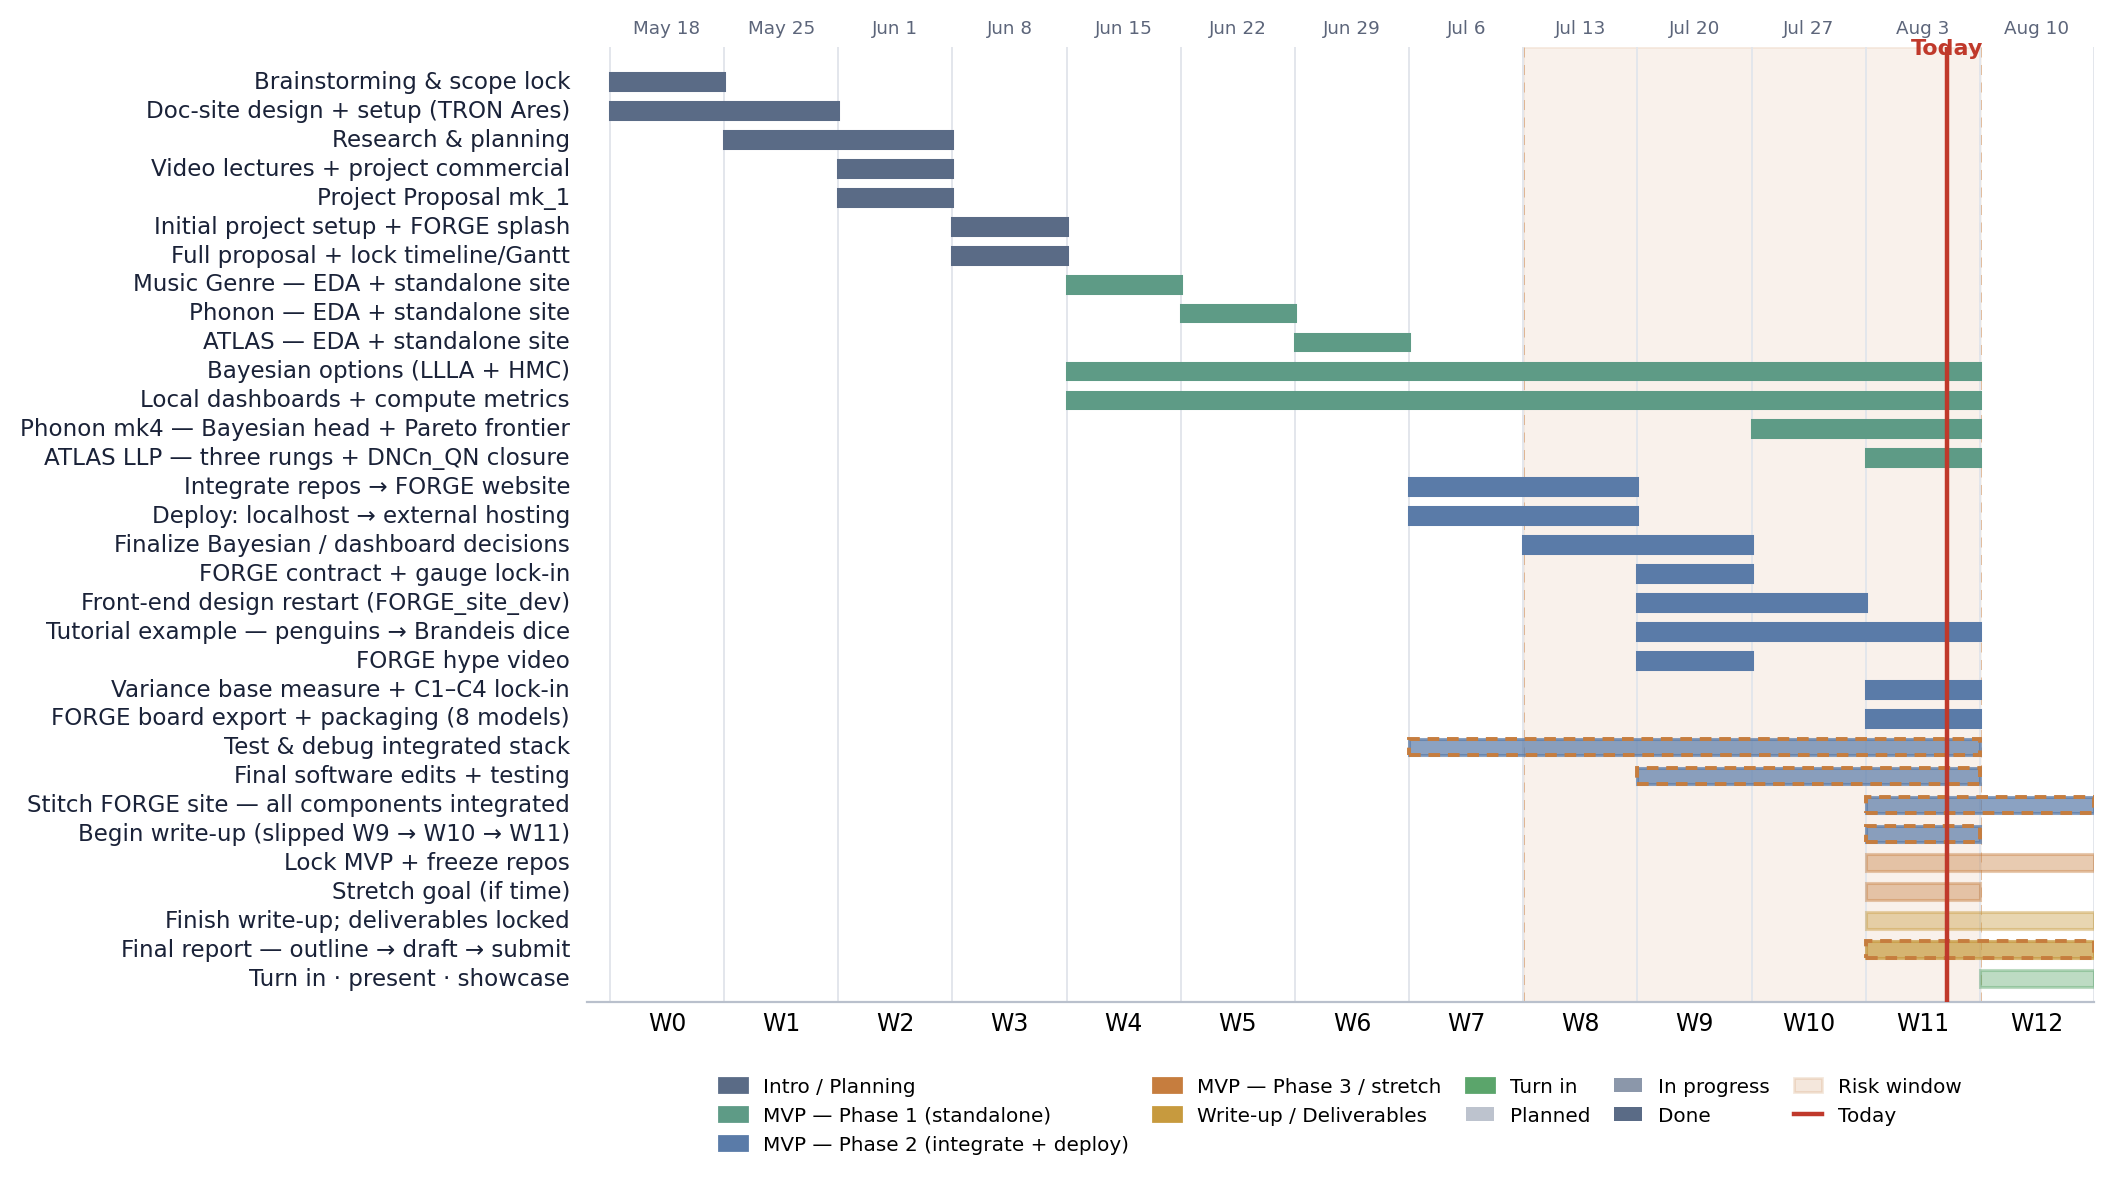
\includegraphics[width=\linewidth]{gantt_chart.png}
\caption{FORGE project Gantt (snapshot). Bars span the weeks each task is active and are colored by phase (Intro/Planning, MVP Phase~1--3, Write-up/Deliverables); fill density encodes status (planned / in progress / done); the shaded band marks the risk-management window (W8--W10) and the vertical line marks ``today''. Live version: \href{https://n-herling-mk1.github.io/INFO_698_documentation/index.html\#gantt}{n-herling-mk1.github.io/INFO\_698\_documentation \#gantt}.}
\label{fig:gantt}
\end{figure}

% =====================================================================
%  5. WERE THE GOALS MET?
% =====================================================================
\propsec{5}{Final Project --- Final Stats}
\preparedby
\newsection

Sections~1--4 above are the approved proposal, carried forward unchanged so that
the commitments and the outcomes sit in one document. Everything from here to
Section~9 is new. This section closes the loop on the proposal: \S5a marks the
deliverables met and unmet, \S5b records how the instrument's own numerical
contract evolved under development, and \S5c gives the insights --- research and
design --- that the build produced. Sections~6--8 then give the instrument, the
measurements, and what they support.

\propsubsub{5a Deliverables --- met and unmet}

Table~\ref{tab:deliverables} takes the feature list of Section~3 (Table~5) as it
was written and marks each line against what was delivered. Table~\ref{tab:goals-proposed}
does the same for the three project-level goals.

\begin{widetable}
\boardstretch\boardfont
\begin{tabularx}{\linewidth}{|c|W{0.92}|N{0.42}|W{1.66}|}
\hline
\hL{\#} & \hC{Feature (as proposed)} & \hC{Status} & \hC{As delivered} \\ \hline
\multicolumn{4}{|l|}{\textbf{MVP --- phase~1}} \\ \hline
F1 & Preloaded multi-domain baselines & \vyes & Eight models across three domains, all documented and loading through one common interface, with a click-through tutorial alongside them. \\ \hline
F2 & Deterministic\,$\leftrightarrow$\,Bayesian toggle & \vyes & Delivered. The point estimate is the $\tau\!\to\!\infty$ limit of the same axis, so the two views are one continuum rather than two modes. \\ \hline
F3 & Real-time knob panel & \vcav & Retired in favour of \emph{solving} for the knob. $\tau^{*}$ is set by MacKay's evidence criterion --- the value of $\tau$ that maximizes the marginal likelihood of the training data, found by fixed-point iteration and needing no held-out labels --- so the value a user would have hunted for is computed and shown. The likelihood knob became an offline head sweep; the architecture knob was not built. \\ \hline
F4 & Posterior-geometry visualization & \vyes & Posterior bars with MAP ticks, GGN eigenspectrum, reliability and PIT diagnostics, all in-browser. \\ \hline
F5 & Resource-logging layer & \vret & Not built, and not needed. F5 existed to size the metered cloud tier of F6 --- an always-on rented box plus per-second serverless GPU. The stack redesign removed that tier, so there is no bill to predict and no autoscaling to inform. The compute questions that remained were answered directly by measurement in \S6.6. \\ \hline
\multicolumn{4}{|l|}{\textbf{MVP --- deployed}} \\ \hline
F6 & Cloud deployment & \vcav & Deployed and public-live, but not on a cloud host: the rented tier was removed and the stack is tunnelled off a home box at \$0/month. \\ \hline
\multicolumn{4}{|l|}{\textbf{Stretch --- MCP}} \\ \hline
S1 & MCP server & \vno & Descoped. Declared optional in the proposal and not attempted; the risk window was spent on the metric lock-in instead. \\ \hline
\end{tabularx}
\caption{Feature deliverables of Table~5, marked against what was delivered.}
\label{tab:deliverables}
\end{widetable}

\begin{widetable}
\boardstretch\boardfont
\begin{tabularx}{\linewidth}{|W{1.10}|N{0.42}|W{1.48}|}
\hline
\hL{Goal (as proposed)} & \hC{Met} & \hC{On what evidence} \\ \hline
Deploy inside a hobby-scale hosting envelope, $\sim$\$25/month (Table~\ref{tab:host})
 & \vyes
 & \$0/month. Verified public-live from a second machine; only recurring cost is domain registration. \\ \hline
Turn a point estimate into a full Bayesian posterior --- LLLA fast path, HMC reference
 & \vyes
 & Delivered on all four models at the scope \S3b sets --- a Bayesian \emph{head}: a Gaussian posterior over the last-layer weights, with $\tau^{*}$ set by evidence rather than tuned, plus the exact functionals and per-feature rows that follow from it. \\ \hline
Generalize across heterogeneous domains, not one model
 & \vyes
 & Three deliberately unlike reproductions: CNN classifier, E(3)-equivariant GNN regressor, HEP binary search. \\ \hline
Reproduce each base model to its published or historical reference
 & \vyes
 & Phonon 0.717 vs Chen's 0.70; genre reproduces its native prediction exactly; ATLAS NN1 0.8785 vs $\sim$0.86, NN2 0.9697 vs $\sim$0.945. \\ \hline
\end{tabularx}
\caption{Project-level goals as proposed, and the verdict against each.}
\label{tab:goals-proposed}
\end{widetable}

Three of these need a sentence more than a table cell allows.

\textbf{One model needed work before a posterior was possible; two did not.}
Genre and ATLAS already ended in a linear layer --- one feeding a softmax, the
other a sigmoid --- which is exactly the map a Laplace approximation needs, so
the posterior was placed on the network as trained. The phonon network has no
such layer. Its final operation is an equivariant convolution that contracts
hidden features against edge spherical harmonics, with no weight matrix standing
between those features and the prediction --- and the closed-form method (LLLA)
needs one, because it works by placing a Gaussian over the weights of a final
linear map and reading the predictive variance off that map. With no such map, there is
nothing for the Gaussian to sit on.

The fix was a \emph{readout head}: a small linear layer trained on top of the
finished network with all of the original weights held frozen, taking a fixed
vector of features as its input and reproducing the network's own output ---
manufacturing the linear map the method requires, without disturbing the model
it is measuring. Here the feature vector is the network's own 51-bin
prediction, so nothing upstream was retrained. The choice pays a second
dividend: because the fitted head is linear-Gaussian, its posterior is exactly
Gaussian --- the same object the closed-form approximation computes --- so
agreement with an HMC reference is guaranteed by construction rather than hoped
for and checked afterwards.

\textbf{Generalization carries a different cost on each model.} On phonon, the
guaranteed agreement has a flip side --- a check that cannot disagree also
cannot inform, so FF2 and its gauge read nothing there, which was accepted
deliberately when that head was chosen. On ATLAS the constraint is dimensional:
a 129-dimensional last layer is a thin channel to carry epistemic signal
through, and its per-feature rows are latent activations rather than named
physics inputs, so FF4 reports which \emph{coordinate} carries the doubt and not
yet which \emph{variable}. On genre the limitation is the benchmark rather than
the mathematics: the reference is the author's own earlier coursework project
rather than an independent published result, so genre shows that the instrument
ports to a third architecture without also testing it against a third party's
number.

\textbf{F3 was retired, and the reader should register it as a deviation.} The
knob answered a question --- \emph{what should $\tau$ be?} --- that the
instrument answers for itself. Across dashboard iterations it kept resolving
into a cluttered surface with little for a user to do: every control moved a
value toward the optimum, and the optimum is what a user wants anyway. Once the
focus settled on the variance readouts of \S\S6.1--6.2, the decision followed:
compute $\tau^{*}$ and hand the user the answer, not the search. \S7.2 backs it
--- on phonon the evidence optimum sits on the accuracy plateau, so the computed
value is what a search would reach. The cost is H3, the proposal's keystone
hypothesis: \emph{steerable} geometry is now evidenced by a measured $\tau$
sweep, not by a user turning a dial. F5 died with the metered cloud tier it
existed to size (\S5c); S1 was never attempted.

\propsubsub{5b Project Evolution --- the FORGE four}

The four numerical capabilities --- the \emph{FORGE four}, written FF1--FF4
throughout --- are not a proposal commitment, and no such set is named in
Sections~1--4. What the proposal commits to is the two-path architecture of
Feature~F3 --- a closed-form LLLA fast path against an HMC ground truth --- and
the three hypotheses H1--H3. FF1--FF4 grew out of those
rather than replacing them: H2, that the fast path agrees with the sampler
within tolerance, is FF2 in embryo, and H3's steerable knob is the $\tau$ axis
along which all four are now read --- though the knob itself was retired once
$\tau^{*}$ could be solved for rather than hunted.

The set was re-cut twice. The first re-cut came once the dashboard wireframe had
introduced four user-facing gauges, and separated what a user \emph{reads} from
what is \emph{computed} to feed it --- which is also what retired a data-sweep
channel that had been carried on the list doing no work. The second and larger
re-cut came with the variance lock of 5~August: fixing the base measure as
variance under the law of total variance turned four independently-motivated
readouts into four operations on a single budget. That is the evolution worth
recording, because it is what made the set closed rather than a list that could
have kept growing.

\begin{widetable}
\boardstretch\boardfont
% Vertical centring: m-columns centre the cell box, arraystretch is dropped to
% 1.0 so it cannot inflate the row asymmetrically, and \ffcell supplies even
% padding. See forge-report.sty.
\renewcommand{\tabularxcolumn}[1]{m{#1}}
\renewcommand{\arraystretch}{1.0}
\begin{tabularx}{\linewidth}{|N{0.34}|W{1.06}|W{1.30}|W{1.30}|}
\hline
\hL{} & \hC{Was} & \hC{Is} & \hC{Metric it reports} \\ \hline

\ffcell{\centering\textbf{FF1}\par split}
& \ffcell{\ffbul{\item the LLLA fast path\item a stand-in for HMC}}
& \ffcell{\ffbul{\item the panel that answers \emph{how much of this doubt is reducible at all?}\item posterior bars, decomposition, reliability diagram}}
& \ffcell{\ffbul{\item $E_k=\varphi^{\!\top}\Sigma_{(k,k)}\varphi$ against $A_k$\item $\mathrm{EAR}_k=10\log_{10}(E_k/A_k)$ dB\item reducibility $E_k/(E_k{+}A_k)$}} \\ \hline

\ffcell{\centering\textbf{FF2}\par verify}
& \ffcell{\ffbul{\item the HMC gold standard}}
& \ffcell{\ffbul{\item a run-gated panel answering \emph{is the fast split honest, and which way does it lie?}\item diagnostic table and trace plots}}
& \ffcell{\ffbul{\item $\varepsilon_k=(E_k^{\mathrm{LLLA}}-E_k^{\mathrm{HMC}})/E_k^{\mathrm{HMC}}$, signed\item fidelity $=100(1-\overline{|\varepsilon_k|})$\,\%}} \\ \hline

\ffcell{\centering\textbf{FF3}\par source}
& \ffcell{\ffbul{\item an eigenspectrum plot}}
& \ffcell{\ffbul{\item the panel that answers \emph{does the reducible part come from data, or from leaked prior?}\item cumulative curvature, bulk vs.\ outlier scatter}}
& \ffcell{\ffbul{\item $c_i=(\varphi\!\cdot\!v_i)^2/(\lambda_i+\tau)$\item prior-leak $=\sum_{\lambda<\tau}c_i/\sum_i c_i$}} \\ \hline

\ffcell{\centering\textbf{FF4}\par locate}
& \ffcell{\ffbul{\item per-feature posteriors\item blocked on two candidates}}
& \ffcell{\ffbul{\item the panel that answers \emph{which inputs carry the reducible doubt, and how much each?}\item feature-marginal table, correlation heat map}}
& \ffcell{\ffbul{\item $a_k=\varphi_k(\Sigma\varphi)_k$, with $\sum_k a_k=E$ exactly\item concentration $100(1-\mathrm{PR})$}} \\ \hline
\end{tabularx}
\caption{The FORGE four: what each dashboard channel was first conceived as,
what it became, and the number it now reports.}
\label{tab:forge-four}
\end{widetable}

Read down the middle column and the evolution is one move, made four times: each
channel stopped being an object --- a path, a sampler, a plot, a marginal --- and
became a question with a number attached. Read across and the four questions
partition one budget between them, which is why the set closed at four. Where
each channel stops reading is argued in \S8, and the two channels not yet
reading everywhere are carried into \S9.

\propsubsub{5c Project Insights}

\textbf{Research.} Four findings survive the build, each argued with its
measurements in \S7 and its consequences in \S8. \emph{The ratio is a field, not
a number} --- reporting epistemic-to-aleatoric along the axis a domain already
resolves turns a scalar into an answer in the domain's own coordinates, and the
resolving-axis table of \S6.3 is the transferable object. \emph{Calibration is
not sufficient} --- the H7 head posts textbook-perfect coverage, reports that
nothing is reducible, and is wrong; only an invariance check catches it.
\emph{The frontier is a trade} --- accuracy, exposable epistemic signal, and
calibration move together along $\tau$, so the operating point is a choice on a
measured curve rather than a target hit or missed. And \emph{the honest line}:
the phonon instrument reads 0.664 at its evidence-selected operating point,
below Chen's 0.70; the 0.717 that beats the published figure is read at the
collapse end where the instrument reads nothing. Two outcomes were not committed
to in the proposal at all --- the ABCD closure result, where at fixed distance
correlation the home-brew term buys three times better closure on endcap, and
beating the published phonon baseline outright with a ridge-regularized readout
on a frozen trunk.

\textbf{Design.} The site was rebuilt once, deliberately, and the reason is the
insight. The first architecture followed the proposal literally: three
standalone experiment sites, each driven to ground truth, to be tied together
later. They worked, and the integration exposed the flaw --- three sites meant
three navigations, three vocabularies, and no way to compare one model's
uncertainty against another's, which is the entire point of an observatory. The
front end was restarted in a separate repository as design-only, and the flow
collapsed to one: splash, a single model-select deck, then one dashboard whose
rails do not change between models. The consequence is recorded honestly in the
schedule --- the Week-6 milestone as worded, ``all three standalone sites
functional,'' is \emph{superseded} rather than met, because the standalone half
of it was absorbed at the Week-9 scope narrowing. The second lesson is cheaper
to state and was more expensive to learn: the deployment target moved from a
rented always-on box to a tunnelled home machine, which took hosting from
$\sim$\$25/month to \$0 and removed the usage-estimation work the metered tier
would have required.


%  6. RESEARCH COMPONENT
% =====================================================================
\propsec{6}{Research Component}
\preparedby
\newsection

\propsubsub{6.1 The base measure: variance, not entropy}

The proposal committed to separating what a model does not know from what
cannot be known, without committing to the arithmetic that separates them.
That arithmetic was locked on 5~August 2026, and the lock is the central
methodological claim of this project: \emph{FORGE's base measure is variance,
under the law of total variance, not entropy or mutual information.}

\[
  \underbrace{\operatorname{Var}(y_k \mid x)}_{\text{total}}
  = \underbrace{\mathbb{E}_{\theta}\!\left[\operatorname{Var}(y_k \mid x,\theta)\right]}_{A_k \ \text{aleatoric, irreducible}}
  + \underbrace{\operatorname{Var}_{\theta}\!\left(\mathbb{E}[y_k \mid x,\theta]\right)}_{E_k \ \text{epistemic, reducible}}
\]

Four reasons, each of which cost something to establish. (i) \emph{Regression
works natively.} An entropy split needs a declared likelihood; the phonon DOS
regression has none under plain MSE, so the entropy form is not merely awkward
there, it is uncomputable. (ii) \emph{The number is dimensionless.}
Differential entropy is unit-dependent --- rescaling the DOS axis shifts it by
a constant --- while a ratio of variances is invariant. (iii) \emph{The decibel
becomes literal.} A ratio of variances \emph{is} a signal-to-noise ratio, so
the $10\log_{10}$ convention is derived rather than borrowed by analogy.
(iv) \emph{Mutual information violates axioms} a doubt measure should satisfy:
it is not maximal under complete ignorance, not monotone under mean-preserving
spreads, and not invariant under location shifts. The label-wise variance form has
none of these defects.

The switch was not free and is not presented as free. The July gauge
calibration on the genre bundle was entropy-based and had to be discarded ---
no conversion exists between the two scales. The ``gain at $2\times$ data''
figure changes from 29.29\,\% to exactly 50\,\%, because epistemic
\emph{variance} falls as $1/N$ while the old number was the standard-deviation
rate. The verification gauge changes from a total-variation distance, which
has no natural form for a DOS regression, to a signed relative
epistemic-variance error.

Two readouts sit on top of the split:
\[
  \mathrm{EAR}_k = 10\log_{10}\!\left(\frac{E_k}{A_k}\right)\ \text{dB},
  \qquad
  \mathrm{reducibility}_k = \frac{E_k}{E_k + A_k}.
\]
EAR aggregates as a \emph{ratio of sums}, never a mean of ratios, which
diverges wherever the aleatoric term approaches zero.

\propsubsub{6.2 Four capabilities, one budget}

Under this base measure the four numerical capabilities stop being four
unrelated numbers. Each is one operation on the same variance budget: FF1
\emph{splits} it, FF2 \emph{verifies} the split, FF3 \emph{sources} the reducible
part, FF4 \emph{locates} it.

\boardstretch
\begin{center}\boardfont
\begin{tabularx}{\linewidth}{|c|l|Y|Y|}
\hline
\hL{} & \hC{Role} & \hC{Core quantity} & \hC{Question answered} \\ \hline
FF1 & Split (fast path)
   & $\Sigma=(H_{\mathrm{GGN}}+\tau I)^{-1}$; $E_k=\varphi^{\!\top}\Sigma_{(k,k)}\varphi$ (regression), $E_k=\nabla p_k^{\!\top}\Sigma\nabla p_k$ (softmax)
   & How much of this prediction's doubt is reducible at all? \\ \hline
FF2 & Verify (gold standard)
   & $\varepsilon_k=(E_k^{\mathrm{LLLA}}-E_k^{\mathrm{HMC}})/E_k^{\mathrm{HMC}}$, signed
   & Is the fast split honest, and which way does it lie? \\ \hline
FF3 & Source (curvature)
   & $E=\sum_i c_i$, $c_i=(\varphi\!\cdot\! v_i)^2/(\lambda_i+\tau)$; prior-leak $=\sum_{\lambda<\tau}c_i/\sum_i c_i$
   & Does the reducible part come from data, or from leaked prior? \\ \hline
FF4 & Locate (allocation)
   & $a_k=\varphi_k(\Sigma\varphi)_k=\tfrac12\varphi_k\,\partial E/\partial\varphi_k$, with $\sum_k a_k=E$ exactly (Euler)
   & Which inputs carry the reducible doubt, and how much each? \\ \hline
\end{tabularx}
\end{center}

The dashboard's four user-facing gauges G1--G4 --- a later design artefact than
the proposal, and distinct from the capabilities that feed them --- are read off
these channels, and all four changed value when the base measure changed. G1
(provenance) becomes the epistemic
\emph{variance} share $E/(E+A)$, replacing a mutual-information fraction on a
scale to which it cannot be converted --- the July genre calibration was
refitted, not rescaled. G2 (posterior) becomes the gain at $2\times$ data,
exactly 50\,\%. G3 (attribution) becomes the signed relative
epistemic-variance error of FF2. G4 (genealogy) becomes the concentration of
epistemic variance across features, read as $100(1-\mathrm{PR})$ from the FF4
allocation. There is deliberately no fifth gauge averaging the other four, and
accuracy is not a gauge.

Two consequences are worth naming. First, FF4's allocation is \emph{exact} ---
$E$ is degree-2 in $\varphi$, so Euler's theorem makes the per-feature shares
sum to the total with no residual --- and it must be plotted \emph{signed},
because anti-correlated features contribute negatively and taking absolute
values hides the most interesting rows. Second, this closed a build blocker
rather than adding one: the marginal-block route and the existing
sensitivity code turn out to be the same object up to a factor of
$\varphi_k$, computable from a single matrix--vector product on the cached
$\Sigma$.

The regularization scale $\tau$ is not tuned on test data. It is set by MacKay's
evidence criterion: the marginal likelihood $p(\mathcal{D}\mid\tau)$, obtained by
integrating the weights out of the posterior, is maximized by fixed-point
iteration on $\tau=\gamma(\tau)/\lVert w\rVert^2$ with
$\gamma(\tau)=\sum_i\lambda_i/(\lambda_i+\tau)$ the effective number of
parameters the data actually constrains. On phonon the evidence optimum
$k^*=-4.97$ lands on the accuracy plateau --- an optimum found with no held-out
labels that agrees with the one found using them.

\propsubsub{6.3 EAR is a field, not a scalar}

The single most transferable idea in the project is that the
aleatoric/epistemic ratio should be reported \emph{along the axis the domain
already resolves}, and only aggregated for a headline.

\begin{center}\boardfont
\begin{tabularx}{\linewidth}{|l|l|Y|}
\hline
\hL{Model} & \hC{Resolving axis} & \hC{Reads as} \\ \hline
Music genre & 10 classes & which genres are model-limited vs.\ genuinely confusable \\ \hline
Phonon DOS & energy bin $\omega$ & $\mathrm{EAR}(\omega)$ --- which frequency ranges are data-limited vs.\ physics-limited \\ \hline
ATLAS LLP & signal region & whether an excess is ignorance or background \\ \hline
\end{tabularx}
\end{center}

A global average is not merely less informative here, it is wrong: in the
ATLAS case the overwhelming majority of events are trivially background, so an
unconditioned EAR reports the background and says nothing about the search.

\propsubsub{6.4 Generalization design}

Three reproductions were chosen to be as unlike each other as the schedule
allowed --- a CNN classifier on audio spectrograms, an E(3)-equivariant graph
network regressing a 51-bin spectrum, and a pair of MLPs performing a binary
search on detector data --- so that a result common to all three is a property
of the instrument rather than of one architecture. None of the three, however,
has a known right answer, which is a poor place to debug an identity. Every
structural identity was therefore first checked against a small analytic problem
whose posteriors are available in closed form, and deliberately constructed to
be degenerate --- a planted statistic carrying no information, and an exactly
collinear pair that makes the Gauss--Newton matrix singular on purpose --- so
that the awkward cases were met where the correct answer was already known
rather than discovered in production. That problem was a development instrument
and is not part of the delivered product; the user-facing tutorial is a
click-through of the definitions.

\propsubsub{6.5 Novel domain research: ATLAS closure}

The ATLAS strand is the one contribution here that is not a reproduction. The
production search estimates background with the ABCD method, whose validity
rests on the two discriminants factorizing. The double-DisCo scheme enforces
this with a distance-correlation penalty, $\mathrm{BCE}+\lambda\!\cdot\!
\mathrm{dCor}^2$. To that we add a home-brew closure term, DNCn\_QN, which
penalizes the actual prediction error at the actual cut in units of its own
statistical noise, with a hinge so that it is silent below one standard
deviation. Two fixes were required before it worked: the hinge itself
(the optimizer had been chasing a floor rather than the target) and drawing
cut positions per batch so that training optimizes the same evaluation grid
the gate scores. The two were changed together, so ``the hinge fixed it'' is
\emph{not} established --- an ablation is named as open work in Section~9.

The design idea worth carrying forward is that the ABCD closure statistic can
be planted as a functional, the way the phonon head plants zero-point energy
and heat capacity, so that $\operatorname{Var}\!\left[N_A^{\mathrm{pred}}/
N_A^{\mathrm{obs}}\right]$ falls out of the same covariance block and ``how
uncertain is the background estimate'' becomes a first-class posterior
reading rather than a separate study. The RRM penalty vector of
Appendix~C remains an original and still-experimental metric, used for
selection only and never for reporting.

\propsubsub{6.6 What it costs, and where it stops}

An observatory is only usable if the arithmetic is cheap enough to recompute on
demand, and only honest if it says where it stops. Both were measured.

The cost result is that one top-$k$ Lanczos pass plus two exact traces
($\operatorname{tr}H$ and $\operatorname{tr}H^2$) is sufficient to serve the
epistemic term, the effective-parameter count $\gamma(\tau)$, the log evidence
$\log Z(\tau)$, and the mass preconditioner the sampler needs --- four
quantities off one decomposition. At $d=1200$, taking $k=100$ costs
0.016\,dB of error on the headline reading, which is far below anything a dial
resolves. 
The stopping point is the sampler, not the arithmetic. The measured
last-layer ceiling for a usable HMC reference is around $d\approx2000$, and
the binding constraint there is \emph{mixing}, not compute --- the cost of the
gradient is linear in $d$, but the chains stop moving well before the wall
clock becomes the problem. This ceiling is what sets the head dimensions
across the board: the phonon instrument head at $d=1632$ sits under it, the
high-accuracy configuration at $d=2601$ sits over it, and the ATLAS head at
$d=129$ sits so far under it that the risk runs the other way --- a channel
too thin to carry much epistemic signal at all.

\propsubsub{6.7 What is original here}

Three constructions in this report have no prior art that could be found, and
are presented as original rather than as citations: (i) the
epistemic-to-aleatoric ratio expressed as $10\log_{10}(E/A)$ in decibels,
which is a literal signal-to-noise ratio under the variance base measure
rather than a borrowed analogy; (ii) the signed relative
epistemic-variance error used as the FF2 verification metric, which replaces a
total-variation distance that has no form for a spectrum-valued regression and
which keeps the sign, so the panel reports \emph{which way} the fast path
lies; and (iii) the multinomial density-of-states likelihood with an effective
count derived from the energy grid, which is what gives that regression a
declared likelihood and therefore an aleatoric term at all.

Two further constructions are original but explicitly experimental and are
labelled as such wherever they appear: the DNCn\_QN closure term of
Section~6.5, and the RRM penalty vector of Appendix~C, which is used for model
selection only and never for reporting.

% =====================================================================
%  7. RESULTS
% =====================================================================
\propsec{7}{Results}
\preparedby
\newsection

\propsubsub{7.1 The board}

Eight models were exported to the FORGE bundle format across three domains. Each
reproduces a published or historical reference, then carries one or more
FORGE-readable variants built to expose a posterior.

\boardstretch
\begin{center}\boardfont
\begin{tabularx}{\linewidth}{|W{1.15}|W{1.10}|N{0.63}|W{1.12}|}
\hline
\hL{Model / domain} & \hC{Reference} & \hC{Reference figure} & \hC{Measured here} \\ \hline
\textbf{Phonon DOS} --- E(3)-equivariant GNN, 51-bin spectrum
 & Chen \emph{et al.} (2021), \emph{Direct Prediction of Phonon Density of States with Euclidean Neural Networks}
 & 0.70 frac@10\%
 & trunk retrained from scratch: \textbf{0.711}; MSE 0.0236, JS 0.0596, EMD-1 25.68\,cm$^{-1}$ \\ \hline
\textbf{Music genre} --- CNN on GTZAN spectrograms, $K=10$
 & BEARDOWN (Herling \& Attili, 2025) --- continued work, no external paper; target set in \S3b
 & $\ge$ 0.75 val (cfg\_14: 0.766)
 & 5 models exported ($d=512/384/768/384/768$), best 0.855 val; bundle reproduces native prediction \textbf{exactly} \\ \hline
\textbf{ATLAS LLP} --- two 128-128-1 MLPs, endcap, 27{,}995 events
 & Run-3 MSVtx displaced-vertex search (ANA-EXOT-2025-24); baseline per Schott (2024) as set in \S3b
 & NN1 $\sim$0.86, NN2 $\sim$0.945
 & \textbf{NN1 0.8785} (above reference for the first time), \textbf{NN2 0.9697} \\ \hline
\end{tabularx}
\end{center}

The published phonon checkpoint proved unusable --- it is pickled against a
pre-rewrite version of the equivariance library and its keys no longer match
the current network --- so the trunk was retrained from scratch. Two deviations
are disclosed: float32 rather than float64, and best-epoch rather than
fixed-epoch selection. The second is not cosmetic --- validation accuracy
drifted by $-0.039$ from best to final epoch, so the original fixed-length
schedule would have shipped worse weights.

\propsubsub{7.2 Phonon --- the accuracy-versus-signal frontier}

This is the headline research result. Sweeping the prior scale
$\tau=10^{k}\lambda_{\max}$ across seven decades moves predictive accuracy and
exposable epistemic signal in opposite directions, and moves calibration with
the signal rather than with the accuracy.

\begin{center}\boardfont
\begin{tabular}{|l|c|c|c|c|c|c|c|c|}
\hline
\textbf{$k$} & $+2$ & $+1$ & $0$ & $-1$ & $-2$ & $-3$ & $-4$ & $-5$ \\ \hline
frac@10\% & 0.711 & 0.711 & \textbf{0.717} & 0.691 & 0.684 & 0.678 & \textbf{0.664} & 0.671 \\ \hline
reducibility \% & 0.00 & 0.00 & 0.01 & 0.09 & 0.36 & 1.14 & 2.52 & 3.92 \\ \hline
\end{tabular}
\end{center}

\noindent Across the same sweep PICP95 improves from 0.874 to 0.889 and the PIT
Kolmogorov--Smirnov statistic from 0.256 to 0.156. Two operating points fall
out:

\begin{itemize}[leftmargin=1.4em]\setlength{\itemsep}{2pt}
  \item \textbf{REPORTED} --- $k=0$, rank 51, $d=2601$: frac@10\% \textbf{0.717},
        above both the retrained trunk (0.711) and the published target (0.70);
        reducibility 0.01\,\%, EAR $-38.24$\,dB, PICP95 0.874. The posterior has
        collapsed to a point mass and the instrument reads nothing.
  \item \textbf{INSTRUMENT} --- $k^*=-4.97$ by MacKay evidence, rank 32,
        $d=1632$: frac@10\% \textbf{0.664}, reducibility 2.5--3.9\,\%,
        PICP95 0.889, PIT-KS 0.152. Chosen with no test data.
\end{itemize}

Precision matters here. 0.664 versus 0.711 is 101 versus 108 of 152 materials,
roughly $1.2\sigma$ --- statistically indistinguishable, but not the same number,
and 0.664 sits \emph{below} the published 0.70 benchmark. The correct statement
is that a FORGE-readable head costs accuracy and buys a declared likelihood, an
$\mathrm{EAR}(\omega)$ field, exact zero-point-energy and heat-capacity
posteriors, and named per-feature rows.

Three independent diagnostics flag the high-accuracy end as prior-led rather
than data-led, which is why the dashboard default stays at $k^*$: prior-leak
reads 0.951 at $k=0$ against $\sim\!0.000$ at $k^*$; the gain-at-$2\times$-data
reads 3.44\,\% against $\sim\!43$\,\%; and the EAR field collapses from
16.74\,dB of spread to 7.11\,dB, with all six heads returning the same
most-ignorance-led materials --- the field has stopped discriminating.

\propsubsub{7.3 Phonon --- the head sweep, and the sharpest instrument result}

Six likelihood heads were swept rather than one committed to up front. At the
instrument operating point:

\begin{center}\boardfont
\begin{tabular}{|l|l|c|c|c|c|}
\hline
\textbf{Head} & \textbf{Likelihood} & \textbf{frac@10\%} & \textbf{PICP95} & \textbf{PIT-KS} & \textbf{A-invariance} \\ \hline
H2 planted-diag & Gaussian, planted functionals & 0.664 & 0.889 & 0.152 & PASS \\ \hline
H3 banded & Gaussian, banded $\Lambda$ & 0.664 & 0.886 & 0.149 & PASS \\ \hline
H6 & Gaussian, diagonal & 0.664 & 0.888 & 0.154 & PASS \\ \hline
H4 & multinomial & 0.355 & --- & --- & \textbf{FAIL 184.4\%} \\ \hline
H5 & multinomial + representation floor & 0.355 & --- & --- & PASS 0.2\% \\ \hline
H7 & learned $\sigma^2$ & 0.599 & \textbf{0.951} & --- & \textbf{FAIL 165.6\%} \\ \hline
\end{tabular}
\end{center}

\noindent \textbf{H7 is the result to remember.} It posts PICP95 = 0.951 ---
dead on nominal, the best-calibrated head on the board --- and an EAR of
$-53$\,dB saying nothing is reducible, and it is \emph{wrong}: the
A-invariance referee catches it at 183.9\,\% drift. Calibration alone does not
detect bias contamination. Neither does EAR, which the contamination silently
inflates on the aleatoric side. Only the invariance test catches it. H4 fails
the same way at 165.9\,\%, while H5 --- the same head with a representation
floor --- passes at 0.2\,\%, a sharper argument for the floor than was
anticipated when it was added.

H2 ships. The accuracy spread across the four gated heads (0.559--0.586) sits
inside binomial noise on 152 materials, so calibration is the tie-break: H2 has
the best PICP95 and buys exact functional posteriors and named FF4 rows for a
small PIT-KS cost. H3's banded covariance is worse on both
accuracy and coverage and was dropped --- the correlation correction did not
earn its place.

Five hypotheses were tested and refuted along the way, all recorded: a
peak-normalization penalty (moved accuracy by exactly $+0.000$; the target is
scale-invariant), clipping negative predictions ($-0.059$; a quarter of the
cells are negative and were compensating for high-frequency leakage), a
$\sigma$-weighted loss, a genuinely linear-readout trunk (0.605 --- a 0.106
cost for a real linear last layer), and an invariants surrogate (0.197--0.224,
because the network has no linear last layer at all: its final convolution
contracts hidden features against edge spherical harmonics, and a linear map
on pooled invariants discards exactly that). The net finding is that three
``properly architected'' trunks all lost to using the trained model's own
output as the feature map.

\propsubsub{7.4 ATLAS --- closure, and the referee}

Three rungs were trained on 27{,}995 endcap events: vanilla BCE, plus
double-DisCo, plus the DNCn\_QN closure term. The decorrelation penalty does real
work --- endcap non-closure falls from 223\,\% to 4.8\,\% at $\lambda=5$, a
$46\times$ improvement for 0.002 NN1 and 0.009 NN2 AUC --- then stalls against
the two-sigma gate: dCor keeps falling, closure stops following. A replicated $3\times4\times3$ factorial ($\lambda\in\{2,3,5\}$,
$\mu\in\{0,1,2,5\}$, three seeds) resolves it.

\begin{center}\boardfont
\begin{tabular}{|l|c|c|c|c|}
\hline
\textbf{Endcap operating point} & \textbf{dCor} & \textbf{$|nc|_{\mathrm{med}}$} & \textbf{within $2\sigma$} & \textbf{NN1 AUC} \\ \hline
$\lambda=5$, $\mu=0$ (DisCo only) & 0.0431 & $0.0675\pm0.0179$ & 38.9\,\% & 0.8775 \\ \hline
$\lambda=5$, $\mu=5$ (\textbf{production}) & 0.0430 & $\mathbf{0.0216\pm0.0069}$ & \textbf{88.9\,\%} & $\sim$0.867 \\ \hline
$\lambda=2$, $\mu=1$ (best closure, \emph{fails} dCor gate) & 0.059--0.064 & $0.0213\pm0.003$ & 88\,\% & 0.8692 \\ \hline
\end{tabular}
\end{center}

At the same distance correlation, adding the closure term gives three times
better closure. The mechanism is that the two penalties are not doing the same
job: $\mu$ moves the closure statistic by 20.0 standard errors while moving
dCor by only 2.8, \emph{in the wrong direction}; $\lambda$ moves dCor by 9.1
standard errors. Distance correlation is a global statistic dominated by the
bulk where the events are, while ABCD closure depends on the sparse
high--high corner. One can drive global dependence close to zero and still be
badly off in the corner. The cost is 1.4\,\% relative NN1 AUC (28.8 standard
errors --- small, but real and measured, not zero).

One correction is recorded rather than quietly fixed: an earlier reading of this
board proposed $\lambda=2,\mu=1$ as the operating point on its closure numbers.
That reading skipped the dCor gate, which those cells fail and $\mu$ does not
touch. The substitution result stands as a
statement about \emph{mechanism} --- $\mu$ does more work at low $\lambda$ ---
and does not license lowering $\lambda$ in production.

Barrel is not claimed. Its mid-point closure (0.057) is comparable to the
endcap's, but with 2{,}280 background events against 24{,}850 the error bars
are wide enough to swallow an error the endcap flags; a barrel pass is weaker
evidence than an endcap fail, and the barrel sweep was $n=1$ per cell. Endcap
is the result.

\propsubsub{7.5 Cross-model readings}

\begin{itemize}[leftmargin=1.4em]\setlength{\itemsep}{3pt}
  \item \textbf{The identities hold everywhere.} Across all eight exported
        models the two structural identity residuals read $\sim\!3\times10^{-8}$
        and $\sim\!1\times10^{-15}$; at a complete basis the heat-capacity
        functional is exact to machine precision, retiring an earlier caveat
        about a rank-limited subspace.
  \item \textbf{Last-layer Laplace is structurally over-confident, and the
        signature is identical across domains.} It reads a fraction of the
        parameters --- 1{,}632 of 2.4\,million on phonon --- so model bias is
        absent from the aleatoric term and PIT tails run about 11\,\% against a
        nominal 5\,\%. The same signature appears on genre and on ATLAS. This
        is a property of the method, not of any one model.
  \item \textbf{Packaging.} The full board is 228 files, 6.58\,MB
        uncompressed and 4.54\,MB zipped against a 12\,MB budget, by shipping
        pre-projected curvature terms rather than the full eigenbasis --- which
        took the genre export from 27.10\,MB to 3.17\,MB.
\end{itemize}

\propsubsub{7.6 The deployed observatory}

\screenshotslot{shot_splash}{The splash page. A single strike ignites the
lockup and drops the visitor into the model deck; the site is served at zero
hosting cost from a tunnelled home box.}{fig:shot-splash}

\screenshotslot{shot_deck}{The navigation deck. Four model plates in a
holographic projection; the left rail carries a cathode-terminal help and log
panel that types live facts about whichever model is under the beam.}{fig:shot-deck}

\screenshotslot{shot_forge}{The FORGE dashboard. Left rail selects $\tau$ and
the four capabilities FF1--FF4; the right pane carries the epistemic reading, an
explanation of how that metric fits the whole, and the graph area.}{fig:shot-forge}

% =====================================================================
%  8. DISCUSSION AND INFERENCE
% =====================================================================
\propsec{8}{Discussion and Inference}
\preparedby
\newsection

\textbf{The field is the finding.} If one sentence survives this project, it
is that the epistemic-to-aleatoric ratio should be reported along the axis the
domain already resolves. A scalar EAR for a phonon model is a number; an
$\mathrm{EAR}(\omega)$ spectrum answers a condensed-matter question in
condensed-matter coordinates, and the same restructuring turns the ATLAS
reading from a meaningless global average into a per-signal-region statement.
The resolving-axis table in Section~6.3 is the transferable object.

\textbf{The referee is the real bias detector.} The H7 result is the sharpest
thing measured here, because it is a counterexample to the way uncertainty
work is usually validated. A head that is perfectly calibrated by the standard
test, and that reports confidently that nothing is reducible, is caught only
by an invariance check that neither calibration nor EAR can perform.
Calibration and EAR are each individually blind to the misspecification. This
generalizes past this project: reporting coverage without an invariance test is
not sufficient evidence that a posterior is trustworthy.

\textbf{The frontier is a trade, not a failure.} Accuracy, exposable epistemic
signal, and calibration move together along $\tau$ --- and the direction is
that buying accuracy costs both of the others. The operating point is a
defensible choice on a measured curve. Reporting only the endpoint that
flatters the reproduction would have been the easier document to write and a
worse one.

\textbf{What this instrument cannot do.} Four limits, stated plainly. (i) A
last-layer Laplace posterior sees only the last layer, so model bias never
enters the aleatoric term and every PIT reading runs over-confident.
(ii) Nothing here catches a \emph{wrong} likelihood: if the declared model is
misspecified in the same way everywhere, the fast path and the gold standard
agree beautifully and are both wrong. (iii) Predictive bias contaminates the
aleatoric/epistemic split and arguably belongs on the epistemic side ---
misspecification can masquerade as irreducible noise, at which point EAR
talks the user \emph{out} of fixing the model. This is precisely the failure
the invariance referee exists to catch, and it is the reason the referee is
not optional. (iv) The verification channel is not uniformly available. On phonon's
linear-Gaussian head it is degenerate --- the posterior is Gaussian by
construction, so HMC has nothing to disagree with and FF2 reads nothing there no
matter how carefully it is run. It is genre's categorical head and ATLAS's
Bernoulli head, both non-conjugate, where HMC would actually referee the fast
path, and on both it is unrun.

\textbf{An open question, not a loose end.} The decorrelation and closure
terms are regularizers, not likelihoods --- there is no $p(y\mid x)$ attached
to them. Either the curvature is built from the Bernoulli term alone, with the
penalties affecting only where the mode sits, or they belong inside the
posterior. Their measured coupling on toy data fell below the pre-committed
threshold, so they were excluded --- but that has not been repeated on the real
sample, and the question is unresolved.

% =====================================================================
%  9. CONCLUSION AND FUTURE WORK
% =====================================================================
\propsec{9}{Conclusion and Future Work}
\preparedby
\newsection

FORGE was proposed as a web-hosted observatory that converts a trained
point-estimate model into a Bayesian last-layer posterior and exposes the
uncertainty for inspection at an operating point the instrument selects for
itself. It is deployed, it runs at zero hosting cost, and it
reads four heterogeneous models through one contract. The research
contribution is separable from the product: a variance-based uncertainty
budget in which four capabilities become four operations on one quantity; the
report of that budget as a \emph{field} along each domain's own resolving
axis; a measured accuracy-versus-epistemic-signal frontier with an
evidence-selected operating point that needs no held-out labels; and a
demonstration that calibration is insufficient to detect bias contamination
while an invariance referee catches it.

Named open items, in the order they should be attacked:

\begin{enumerate}[leftmargin=1.6em]\setlength{\itemsep}{2pt}
  \item \textbf{Fill FF2 where it can say something} --- the categorical genre
        head and the Bernoulli ATLAS head, not phonon, whose Gaussian posterior
        makes the check vacuous. It is live on the Bernoulli head and exact on
        the closed-form development problem: it needs running, not building.
  \item \textbf{Route the real curvature into the phonon FF3 panel.} The
        shipped eigenvalue array is a low-dimensional stand-in rather than the
        head's own Gauss--Newton matrix, so FF3's labels and the example
        picker's ordering are not yet trustworthy on that model.
  \item \textbf{Fill the scalar contract for genre and ATLAS}, whose bundles do
        not yet populate the 45-field record.
  \item \textbf{Prove or drop the barrel closure claim} with replicated cells
        rather than $n=1$, and run the hinge-versus-randomized-cut ablation
        that separates the two changes made together.
  \item \textbf{Answer the penalty-in-the-curvature question} on real data,
        and fit a per-network $\tau^*$ rather than reusing one network's.
  \item \textbf{General model ingestion} --- the long-term goal: a researcher
        loads their own trained model, the contract determines which channels
        are applicable, and unavailable channels are declared unavailable with
        a reason rather than silently omitted.
\end{enumerate}

Complete write-ups, the live observatory, the weekly build log, and the full
experiment repositories are linked from the project documentation site given
on the title page.

% =====================================================================
%  5. ETHICS
% =====================================================================
\propsec{10}{Ethics}
\preparedby
\begin{guidance}
Data ethics is a key consideration in any product we create. Include a completed ethics chart (see examples on D2L). For each question, answer Y / N / M (Yes / No / Maybe) for general use and for the data-breach scenario.
\end{guidance}

\noindent\textbf{ATLAS data note.} Whether the ATLAS/CERN detector data underlying the LLP reproduction may be released publicly is still being vetted under the collaboration's data-access and publication policy (with advisor input). If public release is not permitted, the fallback is to keep the data private and release only the model and methodology --- which is sufficient for the FORGE demonstration, since the platform's contribution is the reliability-aware methodology rather than the raw detector inputs.

\renewcommand{\arraystretch}{1.2}
\begin{longtable}{|c|p{9.5cm}|c|c|}
\hline
\hL{\#} & \hC{Question} & \hC{Generally} & \hC{Data Breach} \\ \hline
\endfirsthead
\hline
\hL{\#} & \hC{Question} & \hC{Generally} & \hC{Data Breach} \\ \hline
\endhead
1 & Could a user sell drugs or other illegal items on your platform? & \ynmN & \ynmN \\ \hline
2 & Could a user of your platform engage in sex trafficking? & \ynmN & \ynmN \\ \hline
3 & Could a user sell class notes or cheat on their homework on your platform? & \ynmN & \ynmN \\ \hline
4 & Could a stalker use your project to find someone? & \ynmN & \ynmN \\ \hline
5 & Could your app be used to spy on or track individuals? & \ynmN & \ynmN \\ \hline
6 & Could your app/software access the camera or microphone and record things without users being aware? & \ynmN & \ynmN \\ \hline
7 & If someone uses your platform, could they be re-traumatized or have their mental health impacted in some way? & \ynmN & \ynmN \\ \hline
8 & Could your algorithm promote material that would traumatize or upset individuals? & \ynmN & \ynmN \\ \hline
9 & Would your users be upset if the data you collect was given to someone else? & \ynmN & \ynmN \\ \hline
10 & Could a data leak potentially lead to identity theft? & \ynmN & \ynmN \\ \hline
11 & If your site was hacked, would users potentially lose their job, spouse, or family? & \ynmN & \ynmN \\ \hline
12 & Should there be an age limitation on your product? & \ynmN & \ynmN \\ \hline
13 & Could someone use your product to find, contact, and potentially commit elder abuse? & \ynmN & \ynmN \\ \hline
14 & If the data on your platform was breached, could it be used to blackmail the users? & \ynmN & \ynmN \\ \hline
15 & Does the existence of your project imply that a particular racial group, gender, religion, or other protected category is inherently bad, gross, or unwanted? & \ynmN & \ynmN \\ \hline
16 & Could your product be used to commit hate crimes against a specific group? & \ynmN & \ynmN \\ \hline
17 & Does the primary content of your game or algorithm focus on something considered deeply unethical? & \ynmN & \ynmN \\ \hline
18 & Does your game or software contain race, gender, or other stereotypes? & \ynmN & \ynmN \\ \hline
19 & Could users of your app scam other individuals? & \ynmN & \ynmN \\ \hline
20 & Is your particular algorithm biased toward predicting correctly only for one race, gender, or other group? & \ynmN & \ynmN \\ \hline
21 & Are the users of your project aware of how their data will be used? & \ynmN & \ynmN \\ \hline
22 & What are the possible misinterpretations of your results? & \ynmN & \ynmN \\ \hline
23 & Does the use or purchase of your data potentially contribute to a dangerous group or regime? & \ynmN & \ynmN \\ \hline
24 & Could your virtual reality environment cause injury to the user? & \ynmN & \ynmN \\ \hline
25 & Are your study participants or game players aware that their data will be collected and used? & \ynmN & \ynmN \\ \hline
26 & Does your game or app contain addictive design elements without benefit to the user? & \ynmN & \ynmN \\ \hline
27 & Does your survey contain an aspect of compulsion or unusually large incentive that would command users to take it even to their detriment? & \ynmN & \ynmN \\ \hline
28 & Could your research outcomes harm an individual or entity? & \ynmN & \ynmN \\ \hline
\caption{Data Ethics Chart}
\end{longtable}

% =====================================================================
%  6. APPROVALS
% =====================================================================
\propsec{11}{Approvals}
\preparedby
\begin{guidance}
The project proposal needs the approval of everyone to move forward. If approval is denied, rework the proposal and begin the approval cycle again. Consult the faculty advisor often. After the faculty advisor and team are comfortable with the SOW, only then should it go to the sponsor.

Type the names in the ``Approver Name'' column; written signatures only in the ``Signature'' and ``Date'' columns. Give advisors and sponsors at least 3 business days of lead time. Your instructor signs after grading, if the document passes. Keep the language below.
\end{guidance}

\noindent The signatures of the people below indicate an understanding of the purpose and content of this document by those signing it. By signing this document, you indicate that you approve of the proposed project outlined in this Statement of Work, the division of work, the Ground Rules, and that the next steps may be taken to create a Product Specification and proceed with the project.

\smallskip
\noindent This Statement of Work is self-contained: it is not derived from a separate Product Requirements Document (PRD) and is the governing specification for the FORGE capstone. Any subsequent change is tracked through the Revision History above.

\medskip
\renewcommand{\arraystretch}{1.6}
\begin{tabularx}{\linewidth}{|>{\centering\arraybackslash}p{0.24\linewidth}|c|>{\centering\arraybackslash}X|>{\centering\arraybackslash}p{0.13\linewidth}|}
\hline
\hL{Approver Name} & \hC{Title} & \hC{Signature} & \hC{Date} \\ \hline
Nathan Herling & Project Lead & & \\ \hline
Ken Johns, PhD & Faculty Advisor & & \\ \hline
Nitika Sharma, PhD & Instructor & & \\ \hline
\end{tabularx}

\begin{guidance}
Before you submit to advisor/sponsor for review: refresh the table of contents; verify every table and figure has a number and caption with at least one introductory sentence; clean up white space and page breaks; make sure the revision block is correct.

Before you submit for grading, update the author table below. It need not be 100\% accurate but should give the instructor a good idea of how much each person contributed. For tables and diagrams just put n/a for the word count.
\end{guidance}

\medskip
\renewcommand{\arraystretch}{1.4}
\begin{tabularx}{\linewidth}{|Y|l|c|}
\hline
\hL{Section} & \hC{Author} & \hC{Word Count} \\ \hline
1. Executive Summary & Nathan Herling & $\sim$420 \\ \hline
2 / 2b. User/Market \& Literature Review & Nathan Herling & $\sim$1330 \\ \hline
3 / 3b. Product Features \& Research Deliverables & Nathan Herling & $\sim$1240 \\ \hline
4. Timeline \& Gantt (incl.\ tables/figure) & Nathan Herling & n/a \\ \hline
\end{tabularx}

% =====================================================================
%  7. APPENDIX
% =====================================================================
\propsec{12}{Appendix}
\preparedby

\propsub{A.}{Advisor Engagement}

\propsubsub{Project Team Responsibilities}
\begin{itemize}[leftmargin=1.4em]
  \item The Project Manager will set up and facilitate a weekly call/meeting with the Faculty Advisor. The Project Team will provide weekly status updates including upcoming deliverables, critical issues, and any adjustments to the Project Plan.
  \item Documents will be provided to the Faculty Advisor with adequate time for review and signature, with a minimum review time of 3 days prior to the document due date.
  \item Design files will be provided to the Faculty Advisor as requested in an agreed format.
  \item Support requirements will be clearly requested with the dates required and adequate time for fulfillment.
  \item Modification requests to the Project Plan by the Faculty Advisor will be reviewed and agreed to within 1 week of the request.
\end{itemize}

\propsubsub{Faculty Advisor Responsibilities}
\begin{itemize}[leftmargin=1.4em]
  \item The Faculty Advisor will provide knowledge and expertise to help the group stretch their skills.
  \item The Faculty Advisor will participate in a weekly or bi-weekly call/meeting to review status, upcoming deliverables, priorities, issues, and progress to the agreed Project Plan.
  \item The Faculty Advisor will provide document review, feedback, and approval (or rejection, or approval with contingencies) with adequate time for the team to meet course due dates.
  \item The Faculty Advisor will provide feedback on support requirements, including guidance on design decisions, design files, test plans, test procedures, and test results.
  \item The Faculty Advisor shall provide technical advice and guidance, answering inquiries approximately 1 hour per week.
  \item Modifications to the Project Plan by the Project Team will be resolved and documented within 1 week of the request.
  \item Grade the finalized project using a skill-based rubric.
  \item Attend the project presentation.
\end{itemize}

\propsub{B.}{Ground Rules}
\begin{guidance}
How the team will conduct the business of completing this project. Each team member must sign the Approvals section indicating their acknowledgement of these Ground Rules. Do not remove items from this list, but you may add items.
\end{guidance}

\noindent As a team and as individual team members, we agree to:
\begin{itemize}[leftmargin=1.4em]
  \item \textbf{Stay focused on our objectives and goals.} Each time the team meets, we will clearly define our objectives and desired outcomes at the beginning of the meeting, and politely remind team members if we are getting off track.
  \item \textbf{``Sidebar'' issues that are relevant but not consistent with the immediate objectives.} Create a ``sidebar'' where off-topic but important matters can be listed and discussed later.
  \item \textbf{Listen when others are speaking.} We will listen and consider others' input before adding our own comments.
  \item \textbf{All viewpoints will have an opportunity to be heard.} We will make an effort to get each team member's viewpoint and ensure no one dominates the discussion.
  \item \textbf{Differences of opinion will be discussed respectfully.} We will identify areas of agreement before assessing disagreement, weigh the merits of different opinions, and agree on a process for choosing a direction. All team members will respect and follow the decision.
  \item \textbf{Look for the good points in new ideas.} We will explore the value in each idea as we assess and select our path forward.
  \item \textbf{Focus on the future, not the past.} We will use past experience to inform decisions but focus the discussion on future objectives; blame is counterproductive.
  \item \textbf{Agree upon specific action items and next steps.} At the end of each meeting we will summarize and agree on specific next steps, action items, and assignments.
  \item \textbf{Accountability.} Each member is responsible for their individual assignments and contribution to the team objectives. We will honor our responsibilities and not let our team members down.
\end{itemize}

\propsub{C.}{Exploratory Reliability-Aware Selection Metrics}
\noindent\textbf{Source.} The code and the full BEARDOWN report --- including Figures~6--7 and the metric tables of its Appendix~B --- are public: \urllink{https://github.com/N-Herling-Mk1/INFO_510_Fa25_Final_Proj}{BEARDOWN repository} and \urllink{https://github.com/N-Herling-Mk1/INFO_510_Fa25_Final_Proj/blob/main/_docs/INFO_510_FA_25_Final_Project_Group_7.pdf}{BEARDOWN report (PDF)}.

\smallskip
This appendix collects an author-developed, \emph{exploratory} suite of selection metrics: proof-of-concept rather than established canon, but each resting on a stated hypothesis with initial empirical support. They are used only to \emph{steer model selection during hyperparameter sweeps}, never to report results --- Section~3b's numbers use standard metrics (accuracy, precision/recall/F1, ROC--AUC, ECE) and stay comparable to published baselines, while the selection criterion is free to be more opinionated. The premise: accuracy alone is a poor sweep objective when the target is a \emph{reliable} model, since a configuration can top validation accuracy while being unstable across folds or badly miscalibrated --- exactly the failure mode FORGE exists to expose.

\smallskip
\noindent\textbf{Robust Ranking Metric (RRM) --- the anchor.} For a configuration scored under $k$-fold cross-validation, form a three-axis penalty vector measuring inaccuracy, instability, and posterior uncertainty, and aggregate by Euclidean distance from the ideal $\mathbf{v}=\mathbf{0}$:
\[
  \mathbf{v}=\Bigl(\,1-\bar{a},\ \ \frac{\sigma_{\mathrm{fold}}}{\sigma_{\max}},\ \ \frac{U_{\mathrm{mean}}}{U_{\max}}\,\Bigr),
  \qquad
  \mathrm{RRM} = 1-\lVert\mathbf{v}\rVert_2 .
\]
Here $\bar{a}$ is the mean fold accuracy, $\sigma_{\mathrm{fold}}$ the standard deviation of the per-fold accuracies, and $U_{\mathrm{mean}}=\operatorname{mean}\sqrt{\operatorname{diag}\Sigma}$ the mean posterior standard deviation of the Bayesian head. Selection \emph{maximizes} RRM; it reaches $1$ only for a perfectly accurate, stable, zero-uncertainty model, so nothing can win on accuracy alone while unstable or diffuse. The stability and uncertainty axes are normalized by running sweep maxima ($\sigma_{\max},U_{\max}$, floored at $10^{-8}$) onto a common $[0,1]$ scale; the uncertainty axis is the same posterior signal FORGE visualizes, here turned into an objective. Locked and run in BEARDOWN over two 20-configuration, 3-fold sweeps (\texttt{mk5l}/\texttt{mk5m}).

\smallskip
\noindent\textbf{Preliminary evidence --- non-redundancy.} RRM earns its place only if it carries information the standard metrics do not. In BEARDOWN (Herling \& Attili, 2025, Figs.~6--7) RRM correlated with accuracy at only $r\approx0.62$ ($R^2\approx0.38$, and partly by construction, since accuracy is one of its components), negatively with the uncertainty axes ($r\approx-0.33,\,-0.37$), and was statistically indistinguishable from uncorrelated with an \emph{external} diagnostic not built into it --- off-diagonal confusion noise ($r\approx0.26$, $p\approx0.26$). No single existing metric reproduces its ranking: several high-accuracy configurations scored low on RRM, and some lower-accuracy ones ranked higher. The honest reading is \emph{non-redundant}, not orthogonal --- RRM occupies a distinct direction in metric space rather than re-expressing accuracy. Because Pearson $r$ captures only \emph{linear} association while RRM is a nonlinear (norm) statistic, the planned next diagnostic is distance correlation (dCor, and partial-dCor controlling for the shared accuracy term), which measures dependence without the linearity assumption; the present correlations are exploratory, small-$n$ estimates.

\smallskip
\noindent\textbf{Open question --- the weighting.} Collapsing three heterogeneous axes into one scalar requires a relative weight per axis, $\mathbf{w}=(w_0,w_1,w_2)$, and a fixed choice is both arbitrary and game-able. Because only \emph{relative} emphasis affects the ranking, the weights are normalized to sum to one --- i.e.\ constrained to the probability simplex $\Delta^{2}=\{\mathbf{w}:w_i\ge 0,\ \sum_i w_i=1\}$, the triangle whose three corners place all weight on a single axis and whose centroid weights the three equally:
\[
  \mathrm{RRM}_{\mathbf{w}} = 1-\sqrt{\textstyle\sum_i w_i\,v_i^{2}},
  \qquad \mathbf{w}\in\Delta^{2}.
\]
The locked metric is the equal-weight case --- the centroid $\mathbf{w}=(\tfrac13,\tfrac13,\tfrac13)$ --- which ranks configurations identically to $1-\lVert\mathbf{v}\rVert_2$. Rather than fix $\mathbf{w}$, the intended treatment \emph{samples} it: each weighting is drawn from a Dirichlet distribution $\mathbf{w}\sim\mathrm{Dir}(\boldsymbol{\alpha})$, which lands on $\Delta^{2}$ by construction, so every draw is a valid weighting with no grid or renormalization step. The concentration $\boldsymbol{\alpha}$ sets the coverage pattern: $\boldsymbol{\alpha}=(1,1,1)$ samples the triangle uniformly (no prior preference); large $\boldsymbol{\alpha}$ concentrates draws near the equal-weight centroid (a local sensitivity check); small $\boldsymbol{\alpha}$ pushes them toward the corners (single-axis stress tests). The selection's sensitivity to $\mathbf{w}$ is then reported. This turns ``how independent is RRM of accuracy?'' from a fixed property into a tunable one: the weight slides the metric between an accuracy proxy (mass on $v_0$) and pure reliability (mass off it), letting one choose the weighting that maximizes added information while still selecting good models.

\smallskip
\noindent\textbf{Roadmap.} Beyond RRM the suite includes weight-free global comparisons (rank-aggregation and Pareto-front selection over accuracy and Bayesian reliability; BEARDOWN App.~B) and two candidate fourth axes $v_3$: a false-positive/false-negative--structure term, and, for the ATLAS reproduction specifically, an ABCD background-closure-quality term. All are exploratory and not claims of the main proposal. The configuration this procedure selects is the author-optimized variant (model~2) delivered for each reproduction in Section~3b.

% =====================================================================
%  13. GLOSSARY
%
%  Reference matter, outside the word budget. To add an entry, copy a
%  \glossentry block and keep the list alphabetical by term.
% =====================================================================
\propsec{13}{Glossary}
\preparedby
\newsection

Terms are defined here on the understanding that a reader may meet them out of
order. Where a term carries a measured value in this project, the value and the
section that argues it are given with the definition.

\begin{widetable}
\boardstretch\boardfont
\renewcommand{\tabularxcolumn}[1]{m{#1}}
\renewcommand{\arraystretch}{1.0}
% two columns -> weights must sum to 2.00
\begin{tabularx}{\linewidth}{|W{0.52}|W{1.48}|}
\hline
\hL{Term} & \hC{Definition} \\ \hline

\ffcell{\textbf{MCP}\par\smallskip\textit{Model Context\newline Protocol}}
& \ffcell{An open standard for advertising software functions to a
large-language-model client, so that the client can discover them and call them
as tools rather than a human driving a user interface. FORGE's S1 stretch
(Table~5) would have published the compute functions this way --- a manifest
over the mathematics the dashboard already runs, adding no new science, which is
why the proposal names it first in the descope order (\S3b). Not attempted; see
\S5a.} \\ \hline

\ffcell{\textbf{MacKay evidence\newline fixed point}}
& \ffcell{The rule that sets the prior scale $\tau$ without using held-out
labels. The \emph{evidence} is the marginal likelihood
$p(\mathcal{D}\mid\tau)$, obtained by integrating the weights out of the
posterior rather than fixing them at one value; maximizing it gives the
fixed-point iteration $\tau \leftarrow \gamma(\tau)/\lVert w\rVert^{2}$, where
$\gamma(\tau)=\sum_i \lambda_i/(\lambda_i+\tau)$ is the effective number of
parameters the data actually constrains --- directions with
$\lambda_i \gg \tau$ count fully, directions with $\lambda_i \ll \tau$ barely at
all. Iterating to convergence returns $\tau^{*}$. Because only training data
enters, the operating point is chosen without touching the test set; on phonon
the resulting $k^{*}=-4.97$ lands on the accuracy plateau (\S7.2), so the
value found blind agrees with the value a labelled search would have found.
After MacKay (1992).} \\ \hline

\end{tabularx}
\end{widetable}

\end{document}
